\documentclass{beamer}
\usepackage[T1]{fontenc}
\usepackage[utf8]{inputenc}
\usepackage{lmodern}

\usepackage{color}
\usepackage{graphicx}
\usepackage{amsmath}
%\usepackage{mathabx}
\usepackage[framemethod=tikz]{mdframed}

%%% Package pour faire des tableaux à plusieurs lignes combinées
\usepackage{multirow}

\usepackage[french]{babel}
\frenchsetup{StandardLists=true}

%%% Package pour aligner les colonnes dans un tableau
\usepackage{tabularx}
\usepackage{array}
\usepackage{verbatim}
\usepackage{eurosym}

\usetheme{simple}

\author{H. Commenges & P.Chapron}
\title{Spatial}
\date{}


\begin{document}


\section{Information géographique}

  % Definition du répertoire contenant les images
\graphicspath{{IMAGE/}}

% FRAME Intro
\begin{frame}
%TODO logos

\includegraphics[width=12cm]{Logos.pdf}

\vfill

\begin{center}

\vspace*{1.5cm}

\LARGE
\textbf{Geographic Information}

\vspace*{1.5cm}
 DELHI GIS-R School


\large
9-12\up{th} April 2019

\vspace*{1.5cm}


\textbf{Hadrien Commenges \& Paul Chapron}

{\small

\vspace*{0.1cm}

\url{hadrien.commenges@univ-paris1.fr}

\url{paul.chapron@ign.fr}

}

\end{center}

\end{frame}


% FRAME 
\begin{frame}{Definitions}

\begin{block}{Geographical Information }

Quantitative information, localized in 1, 2, 3 or n dimensions. 
This information is addressed from itls localization point of view.
\end{block}

~

\textbf{Geographical information types:}

\begin{enumerate}
\item Geographical objects (volcanos, railways, forest, etc.)
\item Event occurences (fires, crimes, etc.)
\item Measure points (altitude, temperature, etc.)
\item « Statistics » (population, unemployment rate, etc.)
\item Interaction measures (flows, catchment area, etc.)
\end{enumerate}

\end{frame}



% FRAME 
\begin{frame}{Definitions}

\begin{block}{The question of nature}
The nature of the geographical information is independent from the geographical object, 
 it has to be set by the analyst, according to the research question.
\end{block}

~

\begin{enumerate}
\item Dwellings point patterns (spatial object)
\item Dwellings sales (occurrences)
\item Dwellings prices (measure points)
\item Average price by district (« statistics »)
\end{enumerate}

\end{frame}



% FRAME
\begin{frame}{(1) Geographical Objects }

 Geographical objects come in three types : \textbf{points}, \textbf{lines} and \textbf{areas}. Geographical data analysis focus on their \textbf{geometry} (e.g. length, morphology) and their \textbf{topology} (e.g. neighborhood , distance).

\begin{figure}
  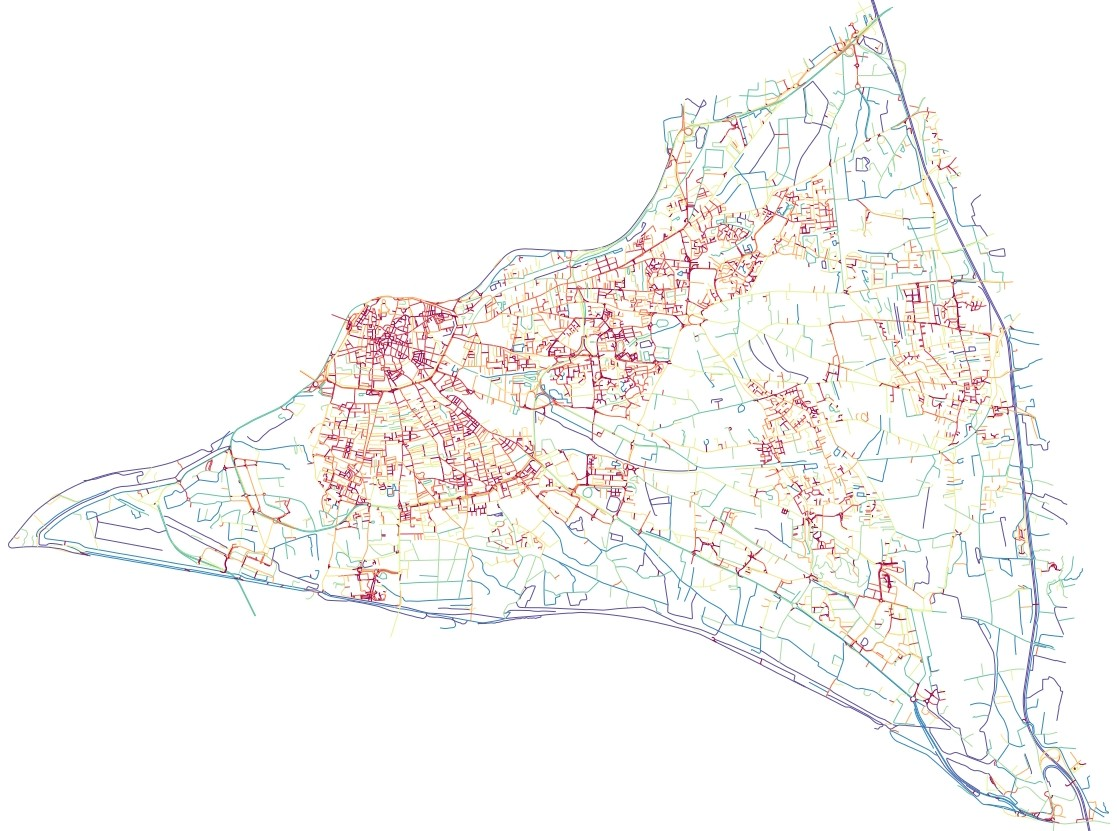
\includegraphics[width=8.5cm]{Morpheo.jpg}
\end{figure}

\end{frame}


% FRAME
\begin{frame}{(2) Event occurence}

 \textbf{Point data}, \textbf{sampled or extensive}, whose localization is under study. 
When it comes to model, localization is  the \textbf{response variable}.

\begin{figure}
  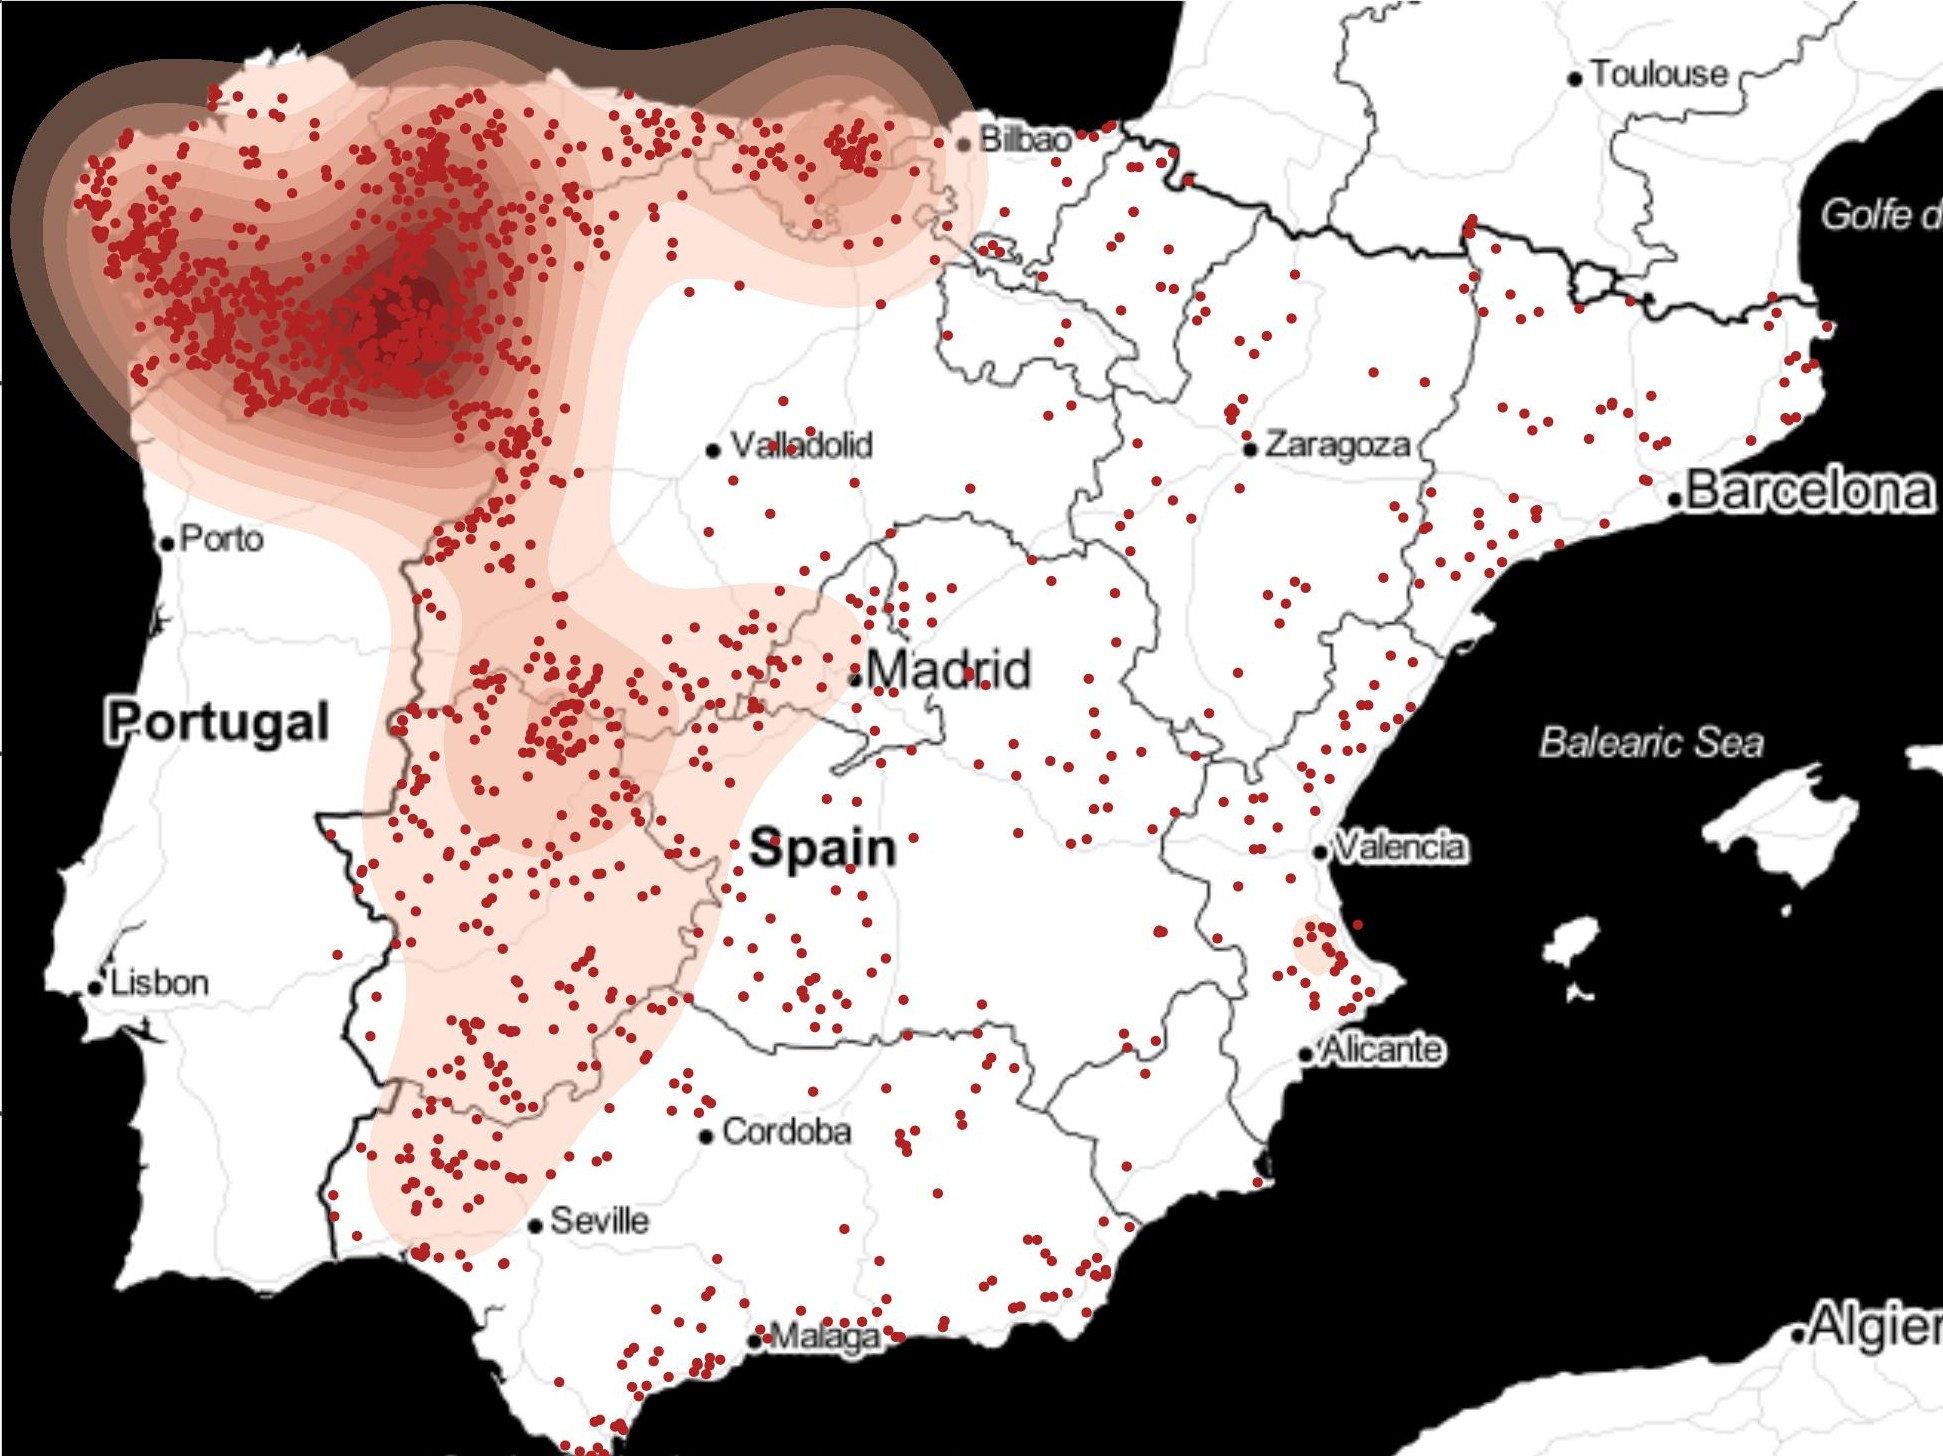
\includegraphics[width=8.5cm]{Incendies.jpg}
\end{figure}

\end{frame}


% FRAME
\begin{frame}{(3) Measure points}

 \textbf{Point data}, \textbf{sampled or extensive}, where a \textbf{value} is associated to each localization.  Phenomenon under study is \textbf{the value variation according to the localization}.

\begin{figure}
  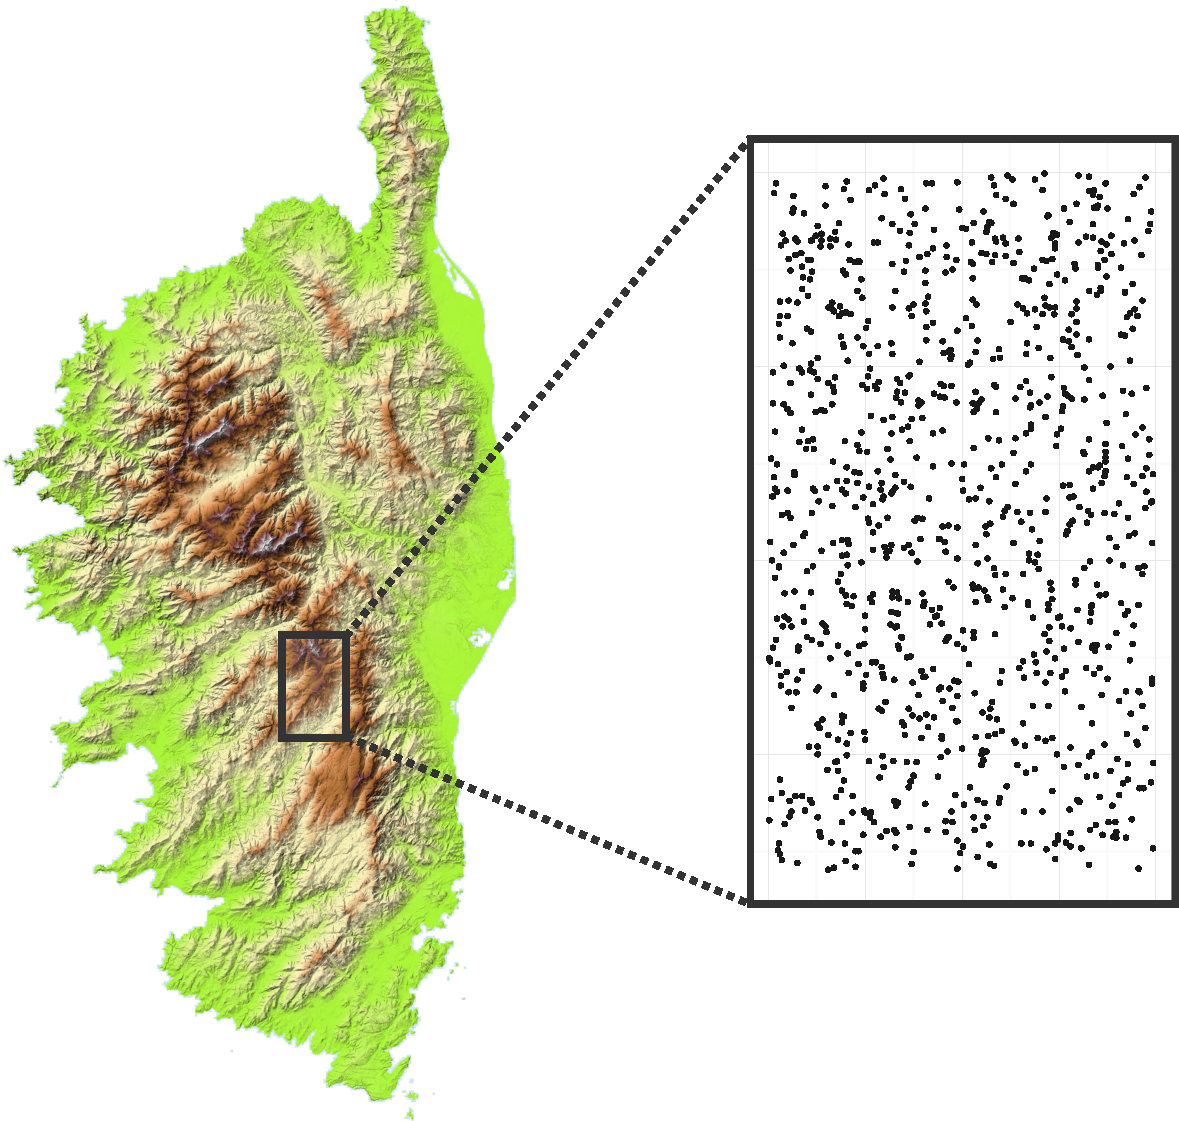
\includegraphics[width=6.5cm]{Corse.pdf}
\end{figure}

\end{frame}


% FRAME
\begin{frame}{(4) Statistics}

«Statistics», from \textit{statista}, «state man»  in italian. \\
\textbf{Zonal extent variables} created from census - \textbf{sampled or extensive} - for territorial management.

Such variables are attributes measured or computed \textbf{within spatial units}.

\begin{figure}
  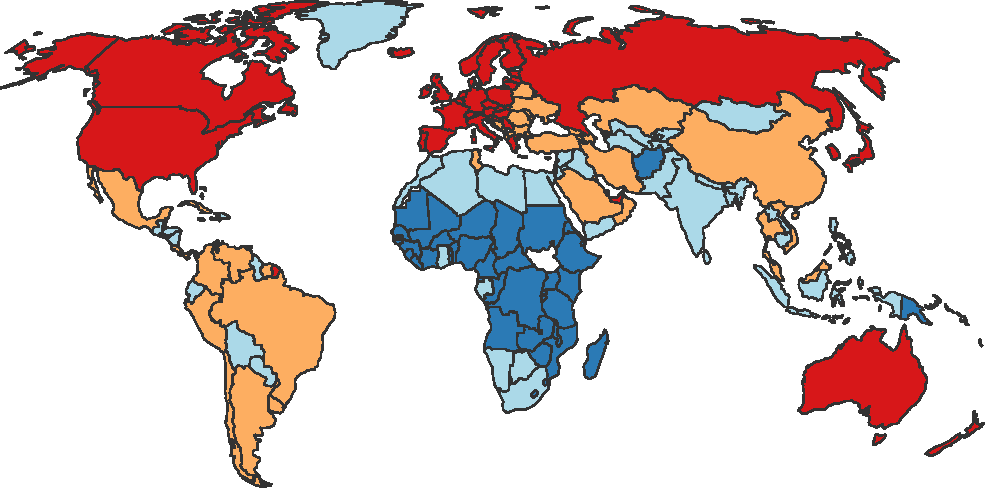
\includegraphics[width=10cm]{World.pdf}
\end{figure}

\end{frame}


% FRAME
\begin{frame}{(5) Interactions}

Interactions concern  \textbf{geographical objects},  \textbf{occurrences} or  \textbf{spatial units} and the \textbf{links} between them.
The object under study is the \textbf{structure} and \textbf{dynamic} of these links (network analysis).

\begin{figure}
  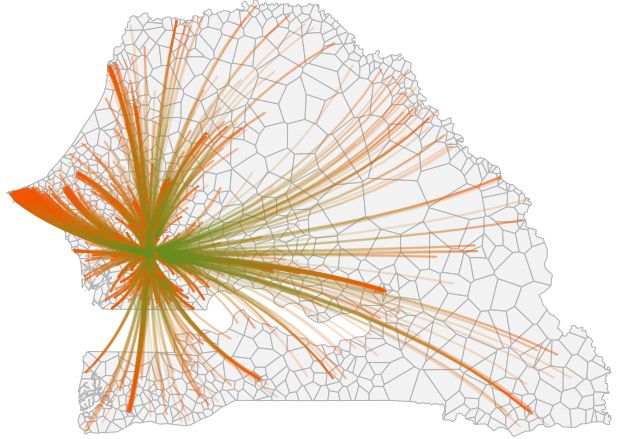
\includegraphics[width=8cm]{Interaction.png}
\end{figure}

\end{frame}




% FRAME
\begin{frame}{Coordinates, areas, distances}

 \textbf{Geolocation} of a spatial entity  depends on:

\begin{itemize}
  \item \textbf{Reference ellipsoid}: Clarke1880, Ellipsoide1909, IAG-GRS80
  \item \textbf{Geoid} : gravity field equipotential surface 
  \item \textbf{Projection}: Mercator, Lambert, Mollweide, etc.
\end{itemize}

 A \textbf{Geodetic system} (or datum) is the combination of these 3 elements (e.g. WGS84)

\end{frame}

% FRAME
\begin{frame}{Coordinates, areas, distances}

%TODO traduire image ?
\begin{figure}
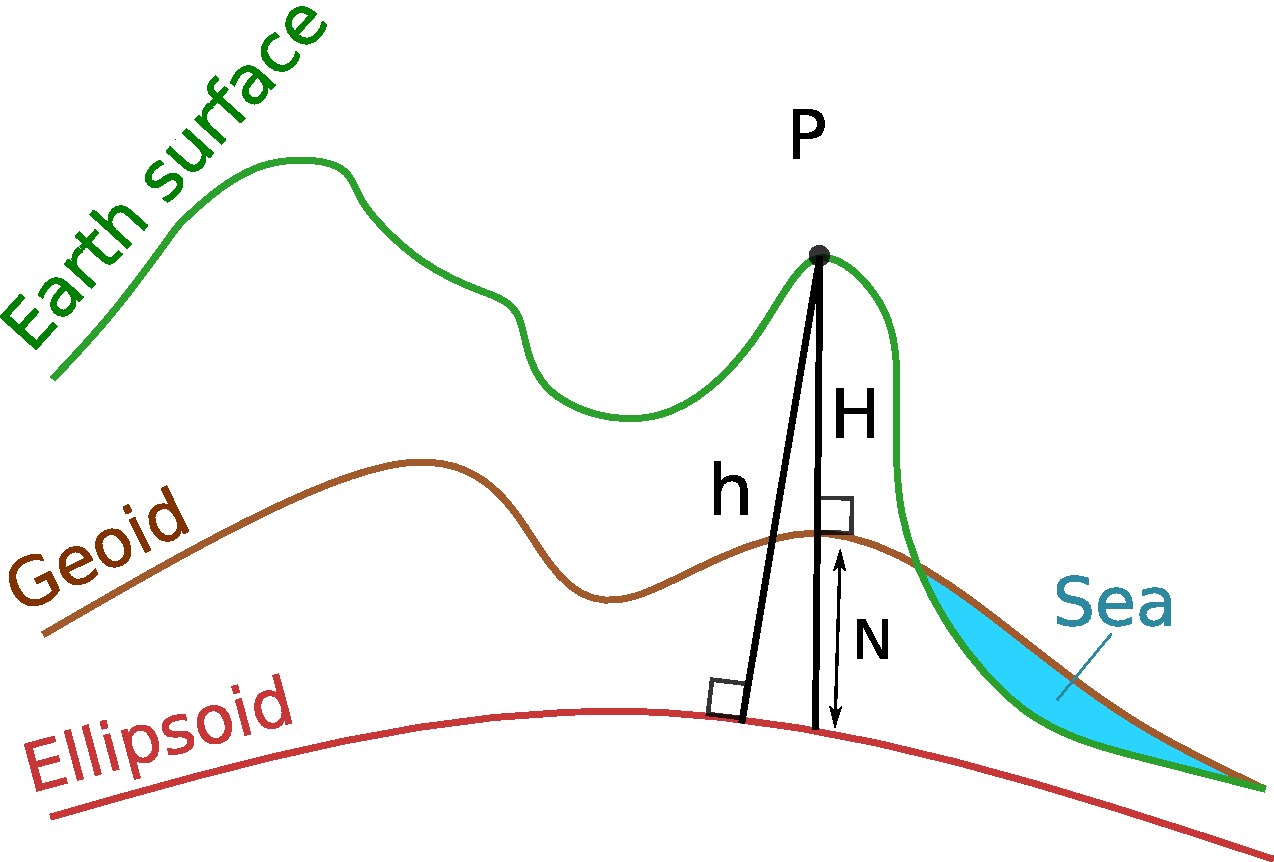
\includegraphics[width=9.5cm]{Geoide_EN.pdf}
\end{figure}

\footnotesize
\emph{Source: ENSG, Les projections et référentiels cartographiques}
\normalsize

\end{frame}



% FRAME
\begin{frame}{Coordinates, areas, distances}

\begin{figure}
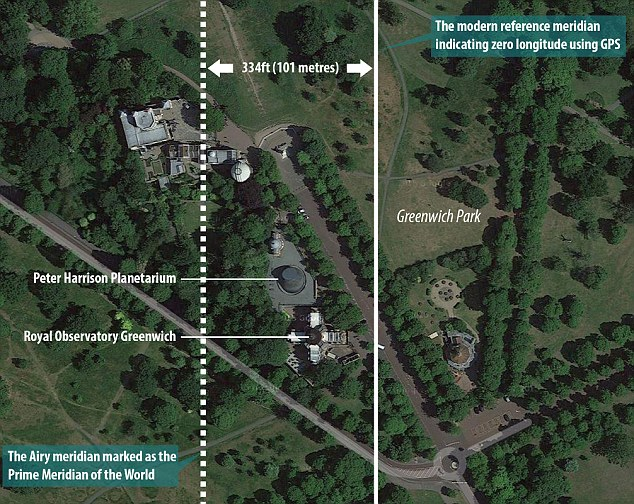
\includegraphics[width=9.5cm]{Greenwich.jpg}
\end{figure}

\end{frame}


% FRAME
\begin{frame}{Coordinates, areas, distances}

A sphere (globe) is a \textbf{non-developable} surface, i.e. cannot be represented as a plane (map) without \textbf{deformation}.

~

Some projections preserve some features  
\begin{itemize}
  \item \textbf{conformal}: conserve angles (shape)
  \item \textbf{equivalent}: conserve areas
  \item \textbf{equidistant}: conserve distances
\end{itemize}

Some others don't. 

~

UTM (Universal Transverse Mercator, conformal) allows almost everywhere an acceptable projection. 

What is the recommandation for India ? Specific ? Kalianpur 5 zones ? 

\end{frame}


% FRAME
\begin{frame}{Coordinates, areas, distances}

\begin{figure}
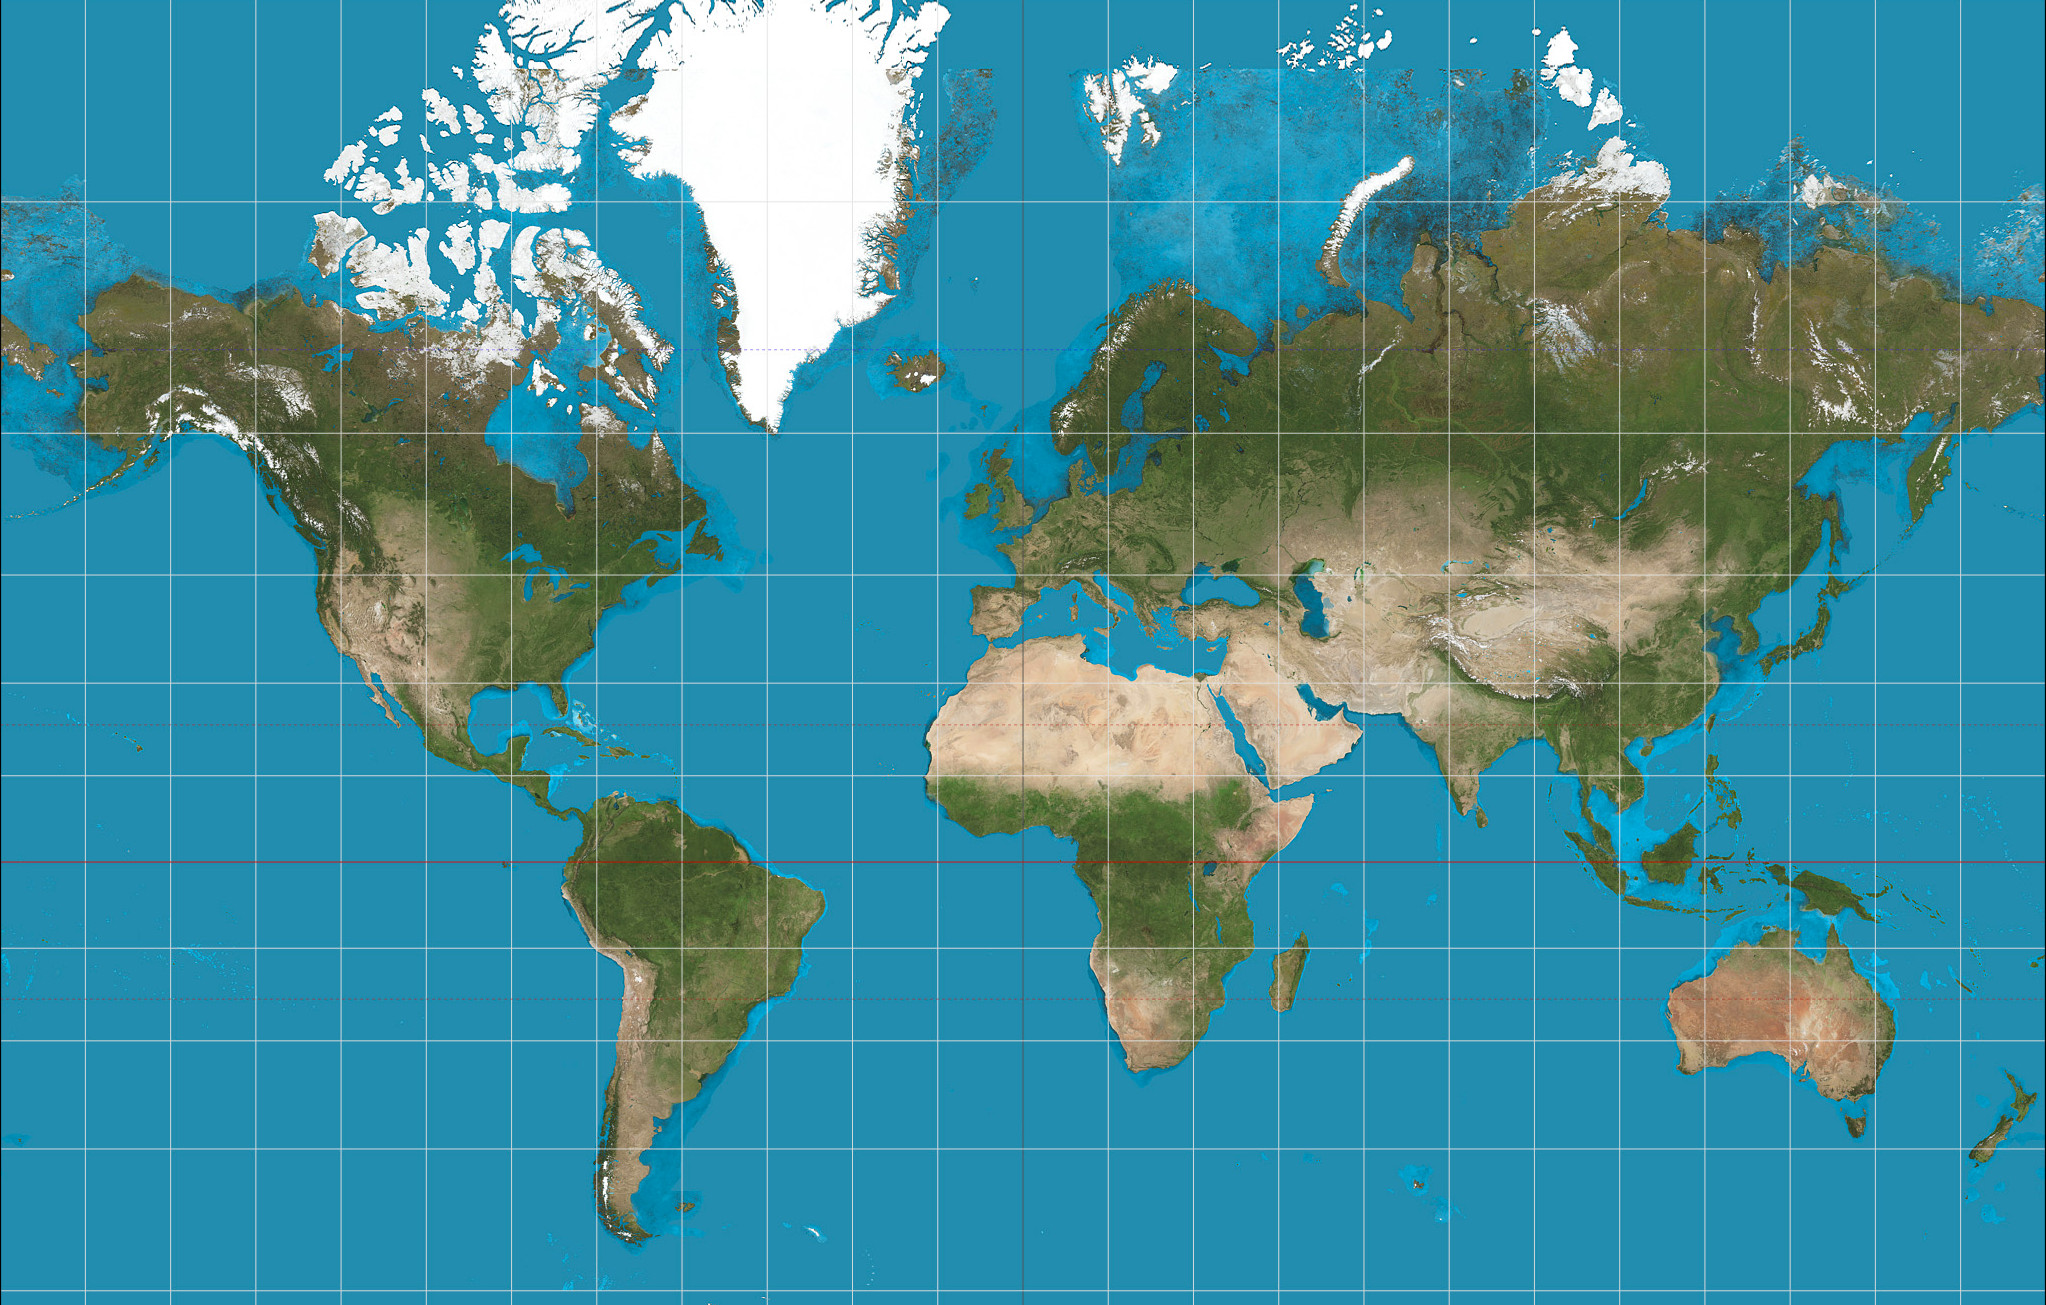
\includegraphics[width=11cm]{MercatorProj.jpg}
\end{figure}

\footnotesize
\emph{Source: Wikimedia, Mercator projection}
\normalsize

\end{frame}


% FRAME
\begin{frame}{Coordinates, areas, distances}

\begin{figure}
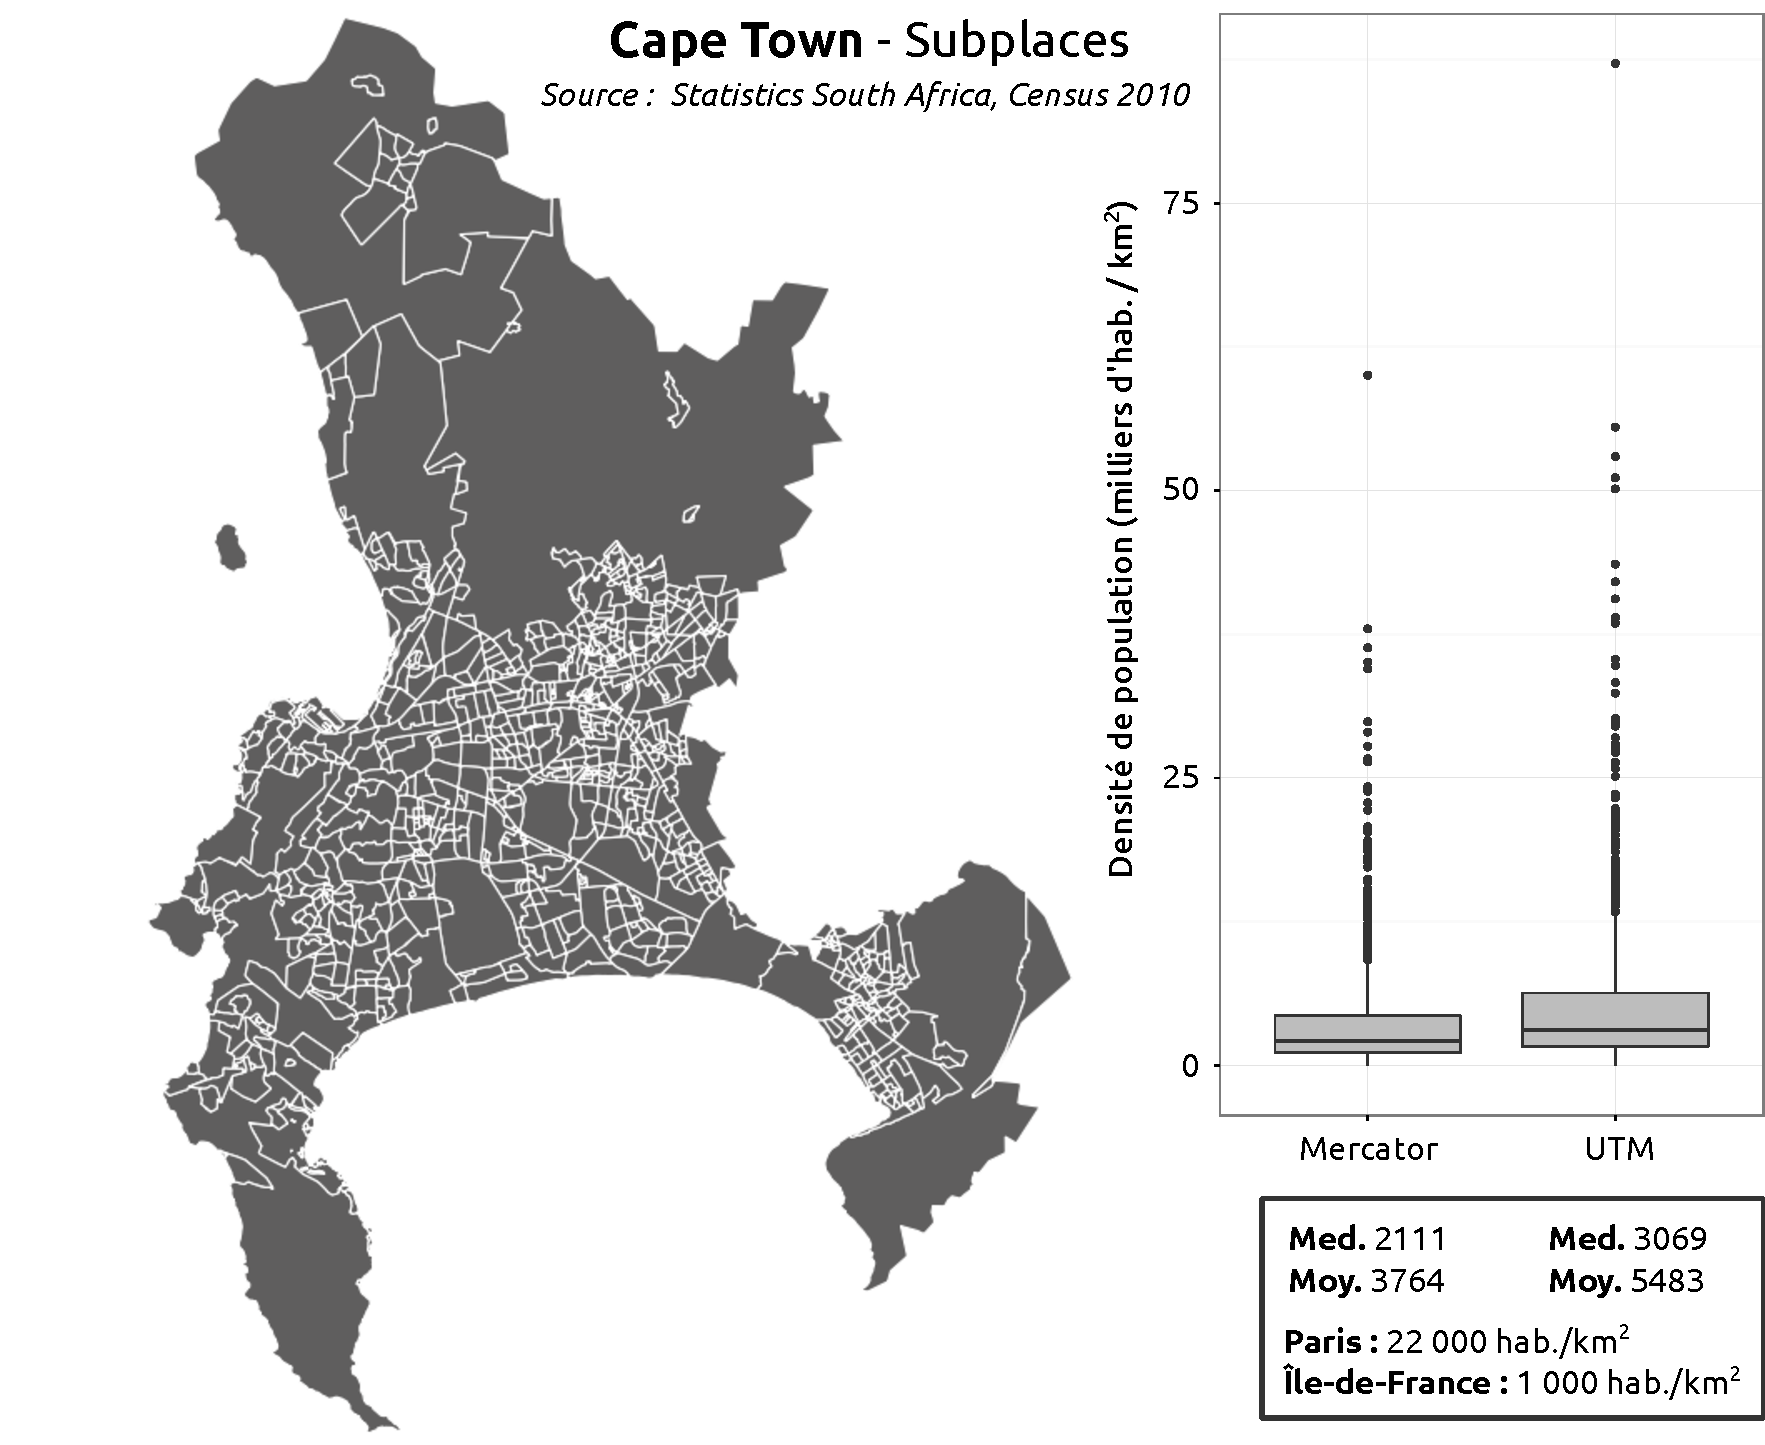
\includegraphics[width=9.5cm]{Projection.pdf}
\end{figure}

\end{frame}


% FRAME
\begin{frame}{Coordinates, areas, distances}

\begin{figure}
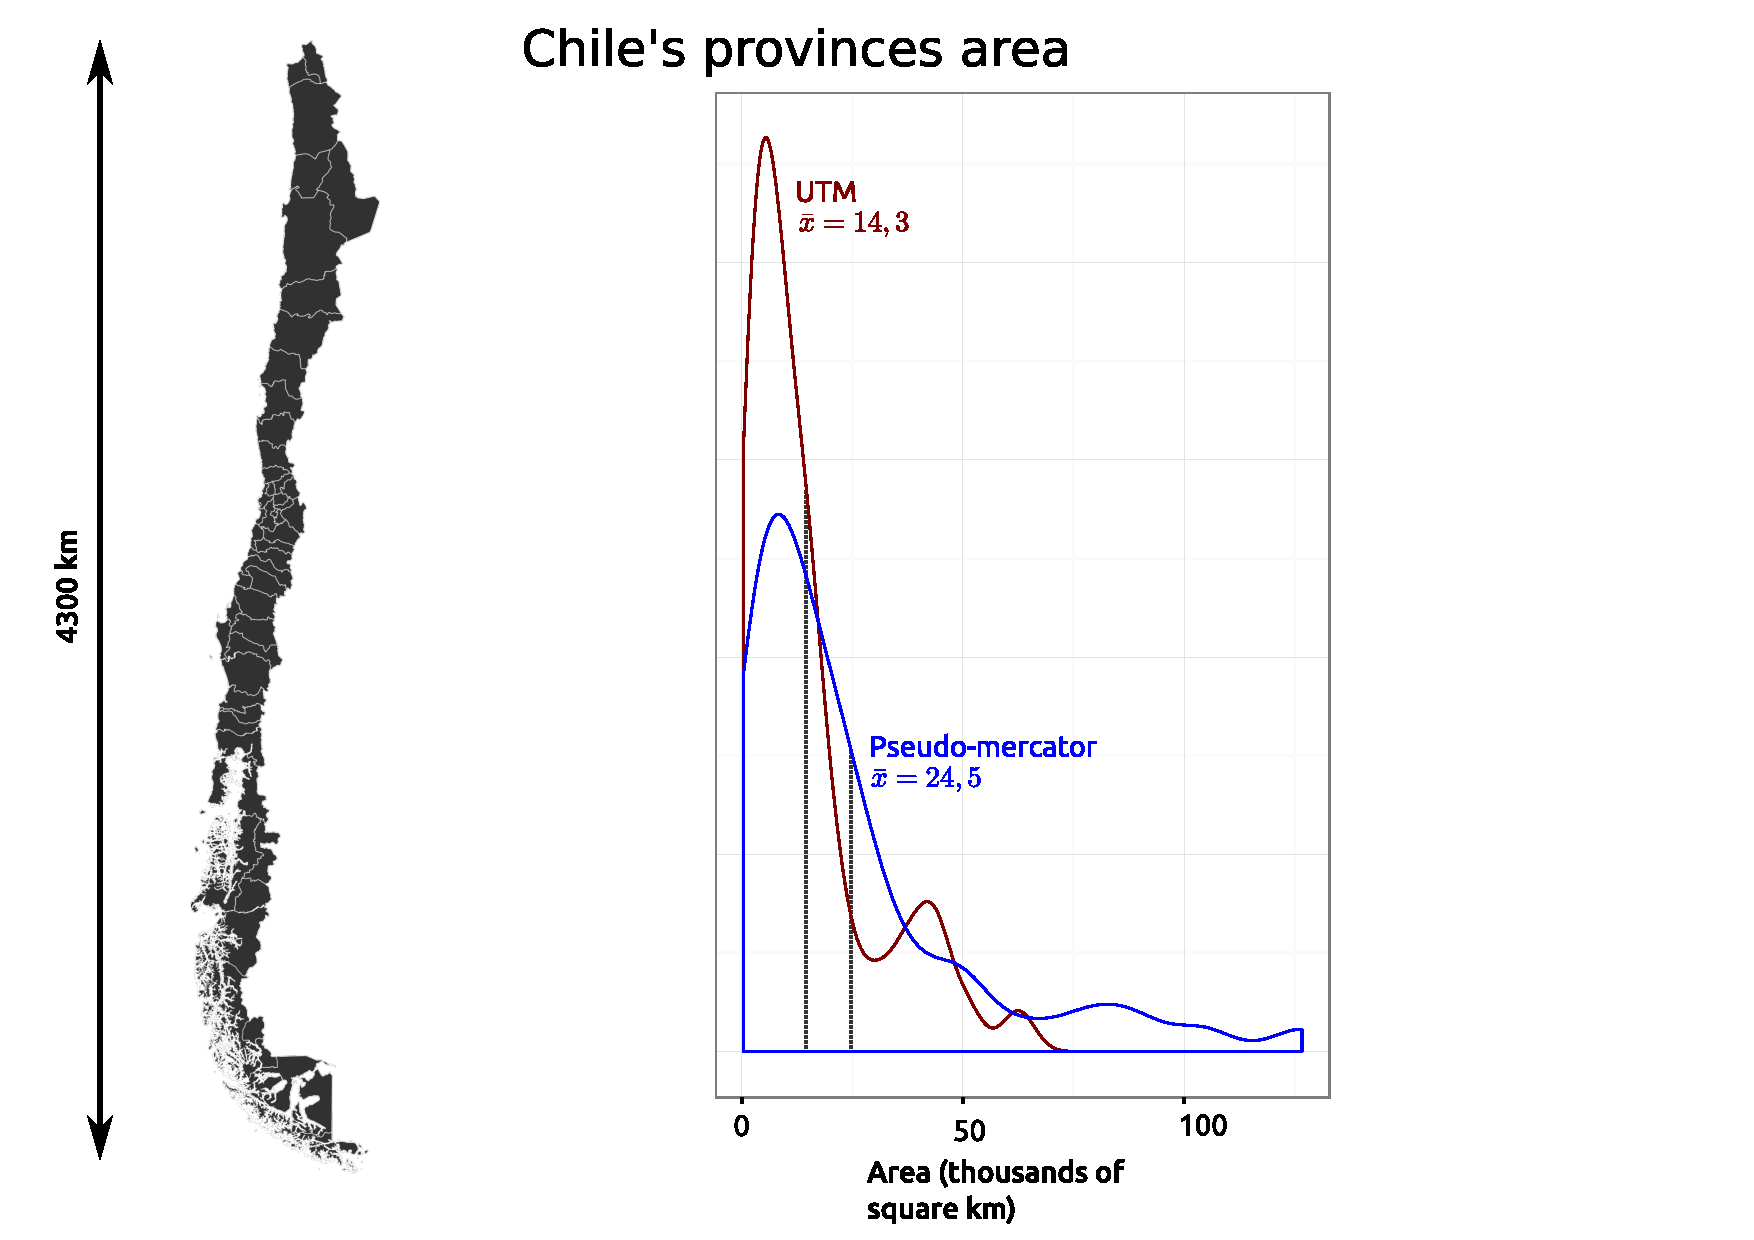
\includegraphics[width=10cm]{ChiliAire_EN.pdf}
\end{figure}

\end{frame}


% FRAME
\begin{frame}{Coordinates, areas, distances}

Basic precautions regarding projection : 

\begin{itemize}
  \item Density $\rightarrow$ any areas alteration ? 
  \item Distance $\rightarrow$ any length alteration ? 
\end{itemize}

~
Regarding  measures :   It depends on the scale ! (and the devices)  

~

GPS-RTK (centimetric precision) or Great-circle distance ? 

\begin{figure}
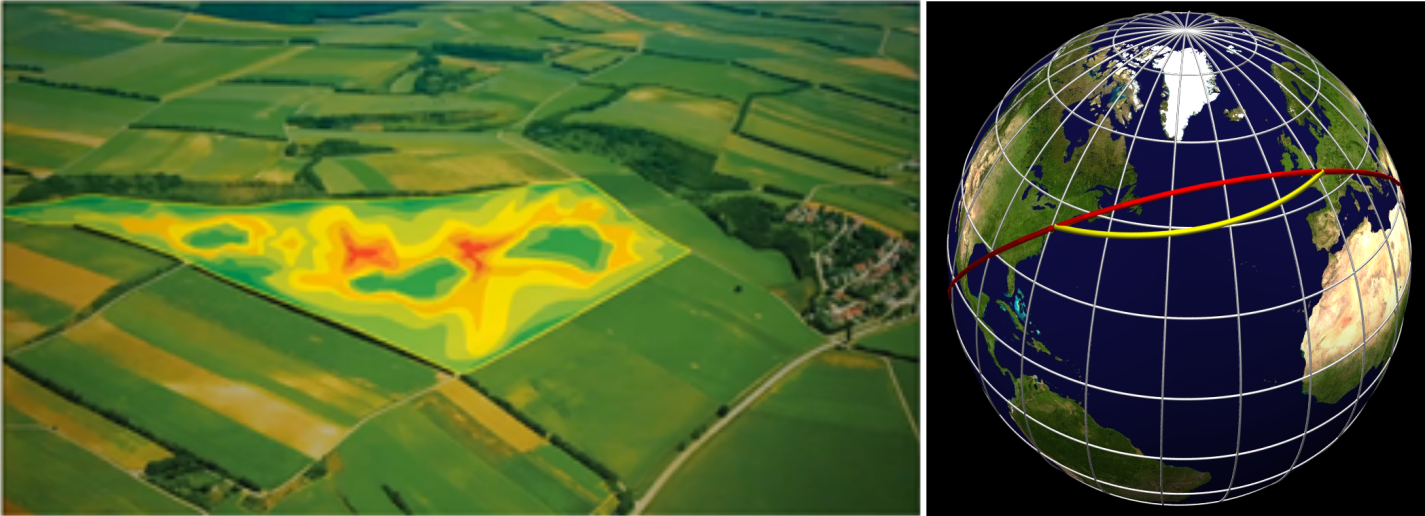
\includegraphics[width=10cm]{Echelle.png}
\end{figure}

\end{frame}


% FRAME
\begin{frame}{Modeling and representation}

\begin{small}
\textbf{to model} (here), is defining \textbf{categories} of objects \textbf{depicting} real-world objects (somehow linked to ontologies).
\end{small}

\begin{figure}
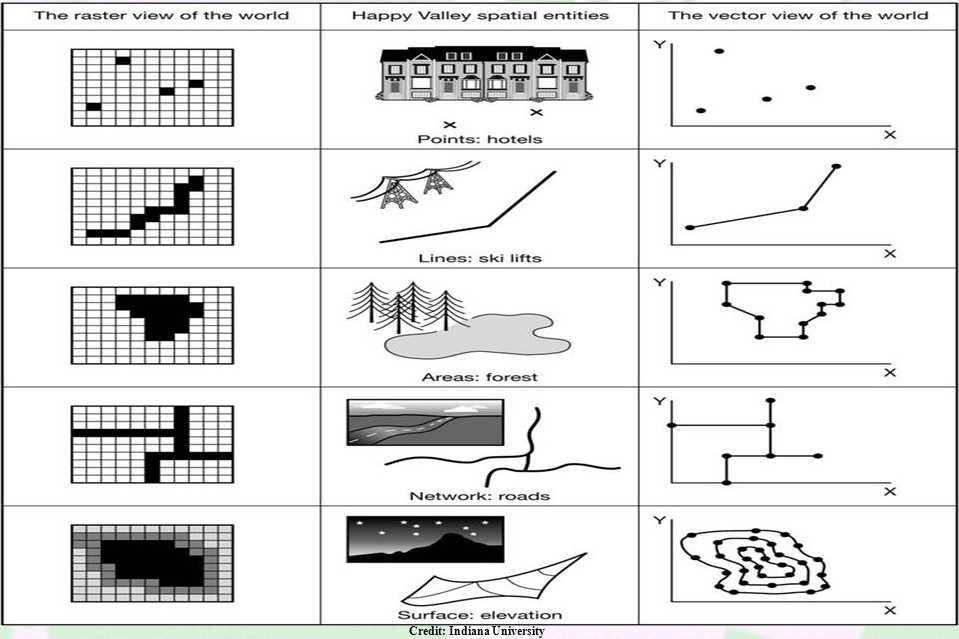
\includegraphics[width=10.5cm]{RasterVector.jpg}
\end{figure}

\end{frame}




% FRAME
\begin{frame}{Modeling and representation}
\textbf{Objects} and  \textbf{Fields}.

\begin{figure}
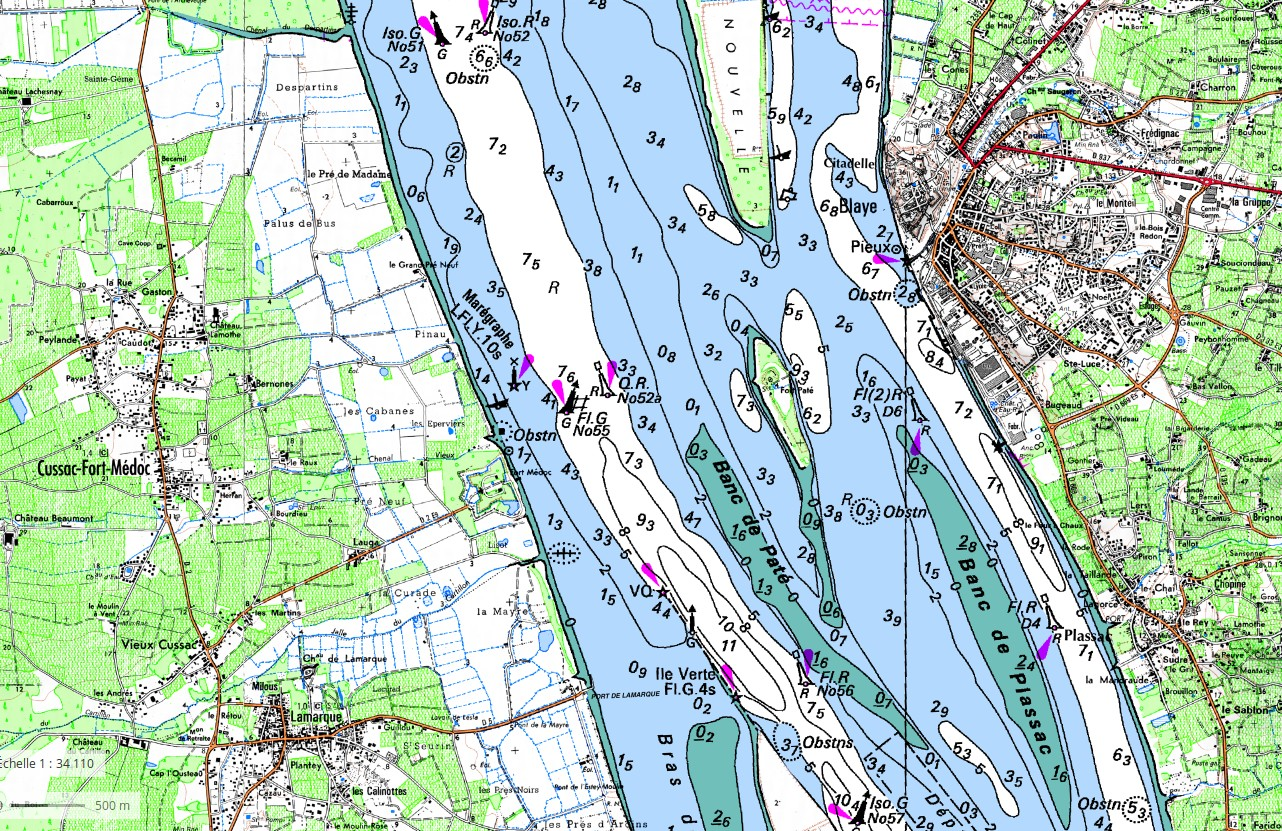
\includegraphics[width=10.5cm]{FortMedoc.jpg}
\end{figure}

\footnotesize
\textit{Sources: IGN and SHOM }
\normalsize

\end{frame}



% FRAME
\begin{frame}{Fields}

\textbf{What does this field represent ?}

\begin{figure}
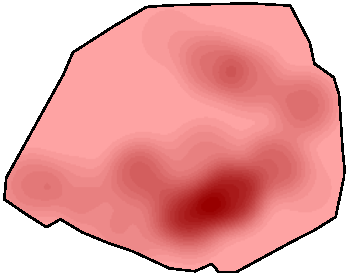
\includegraphics[width=7.5cm]{Champs.pdf}
\end{figure}

\end{frame}


%FRAME 
\begin{frame}{Field definition \& properties}
\begin{center}
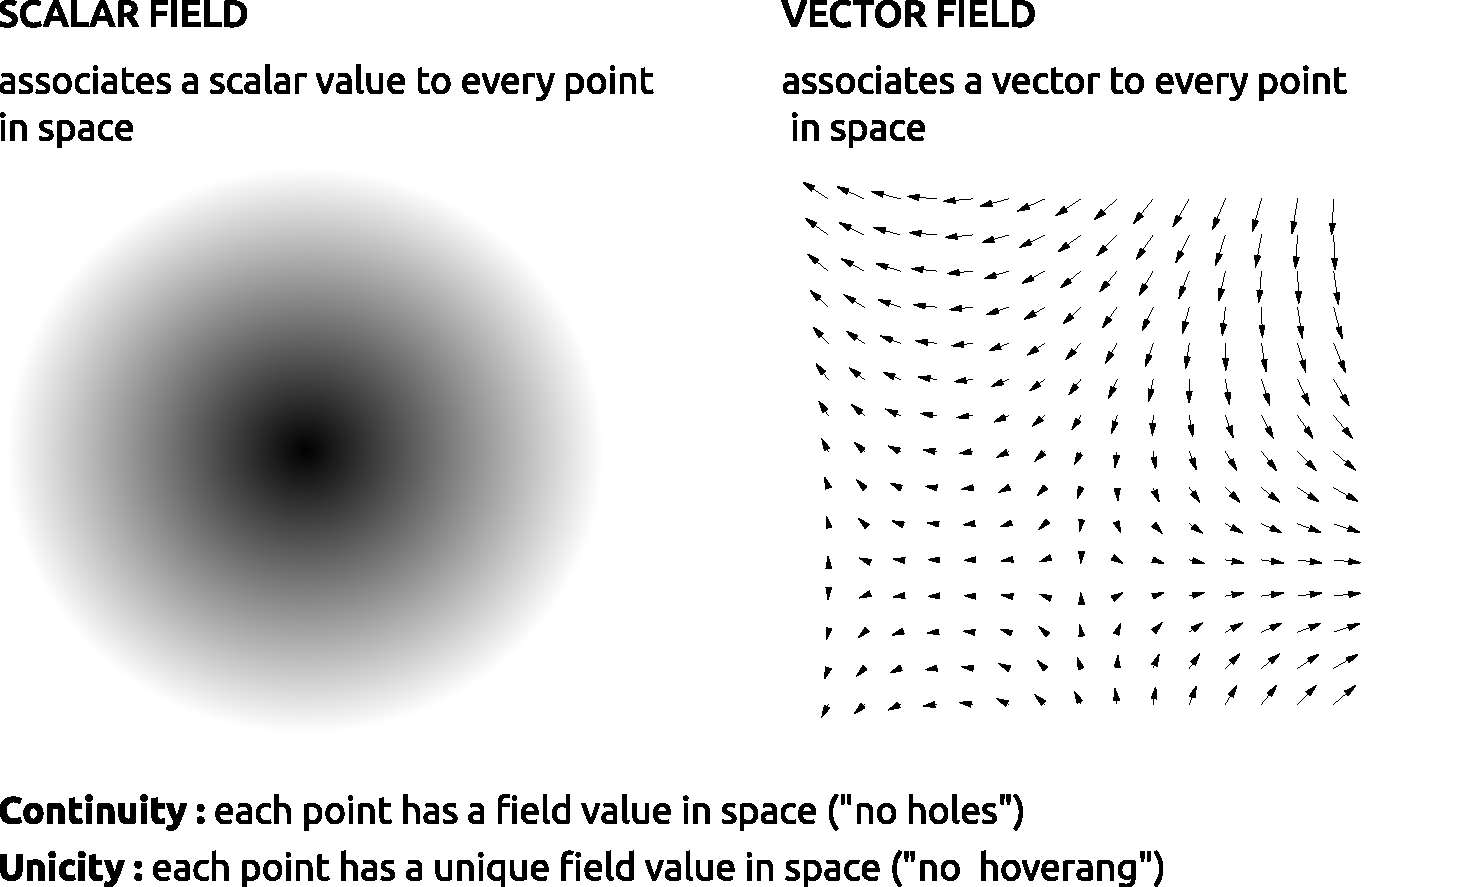
\includegraphics[width=10.5cm]{Champs_EN.pdf}
\end{center}
\end{frame}
% FRAME
\begin{frame}{Fields}

\textbf{Representation modes}

\begin{figure}
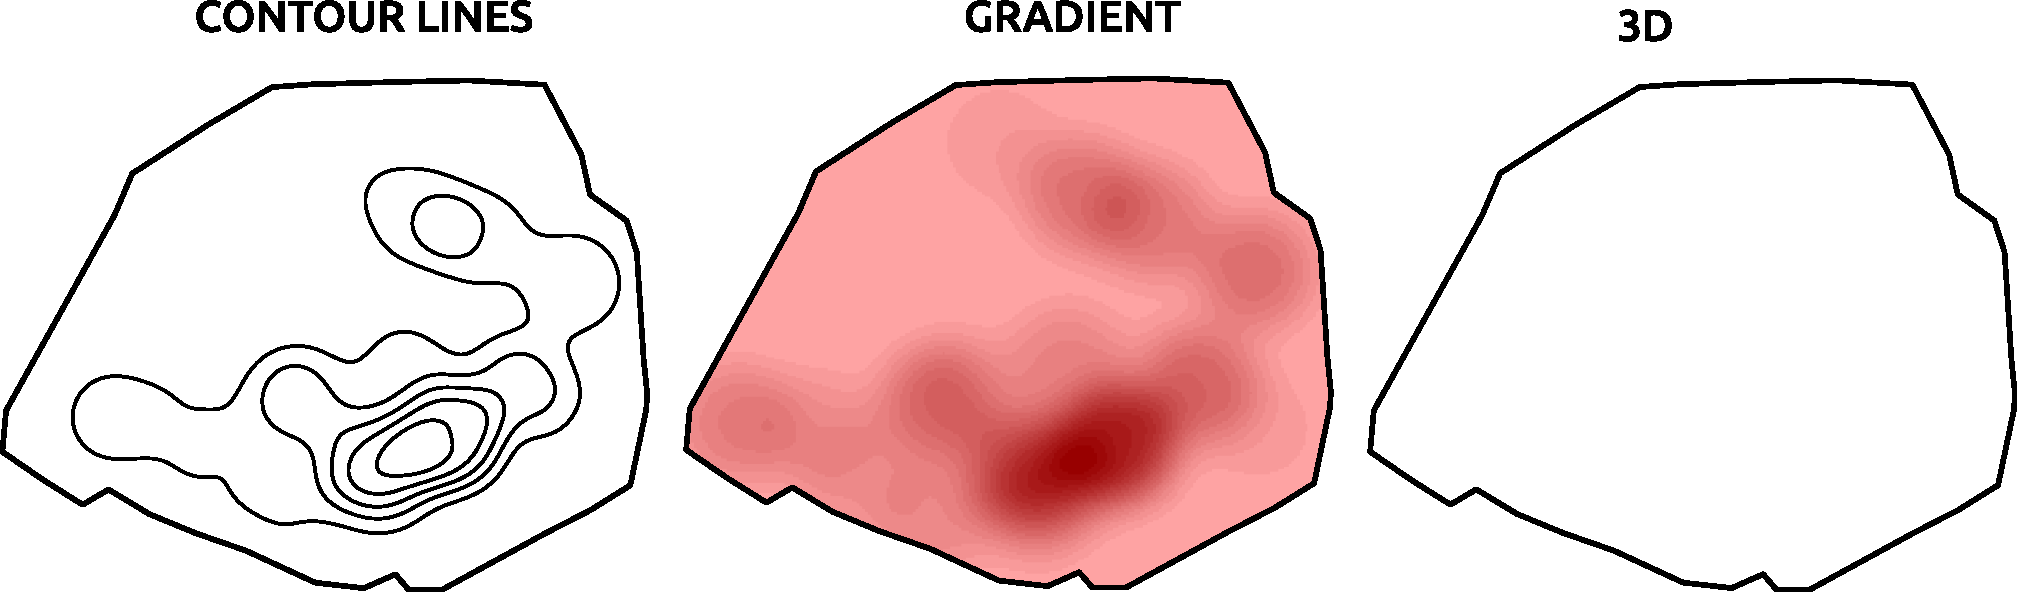
\includegraphics[width=10.5cm]{DeuxSorties_EN.pdf}
\end{figure}

\end{frame}



% FRAME
\begin{frame}{Fields}

\textbf{Representation modes examples}

\begin{figure}
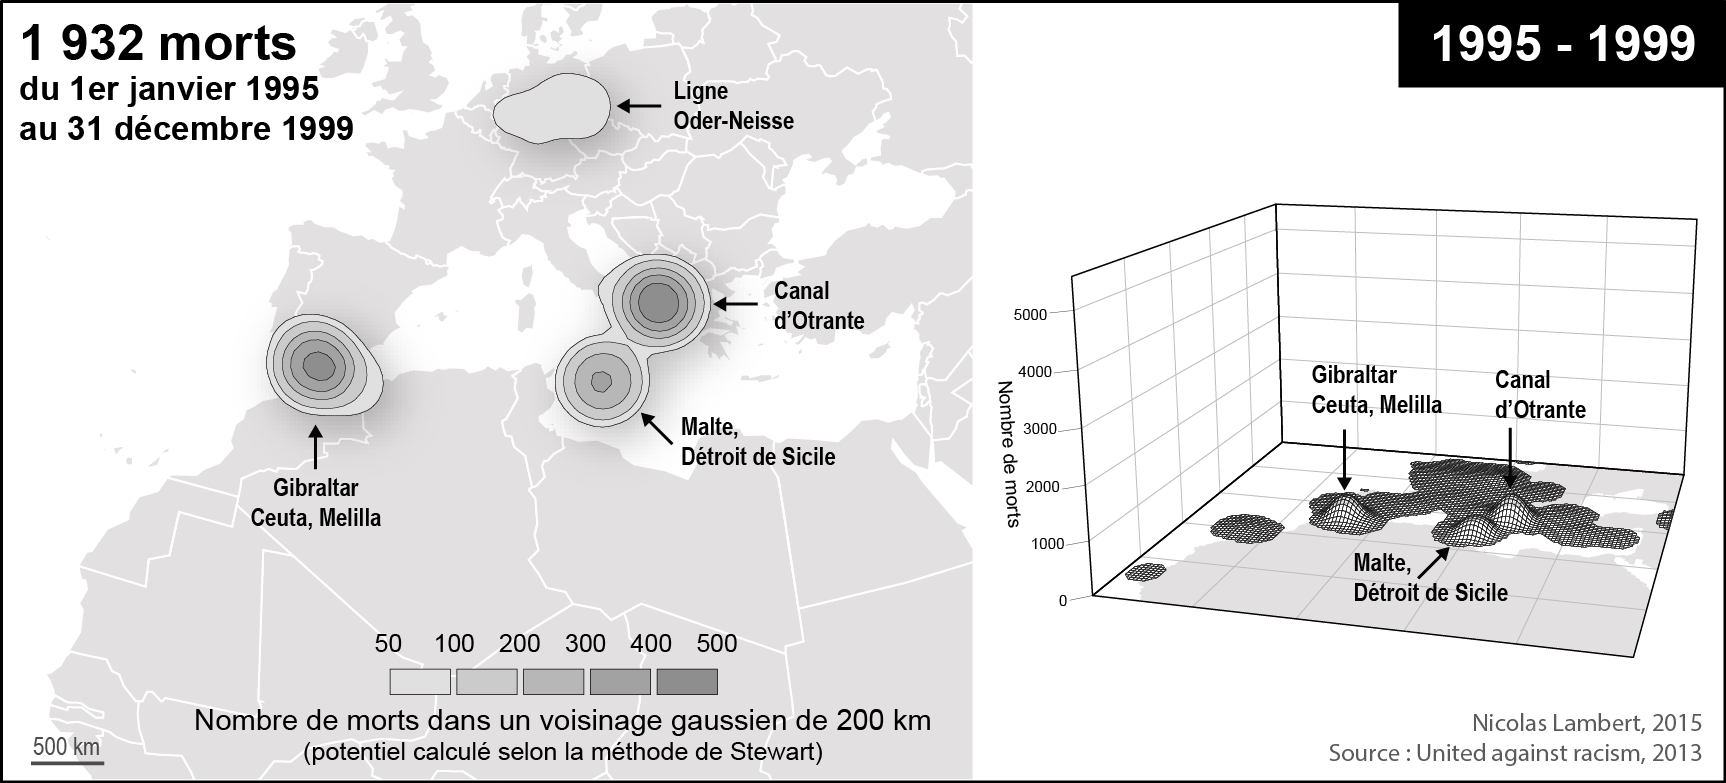
\includegraphics[width=11.5cm]{Migrants1.png}
\end{figure}

\end{frame}

% FRAME
\begin{frame}{Fields}

\textbf{Representation modes examples}

\begin{figure}
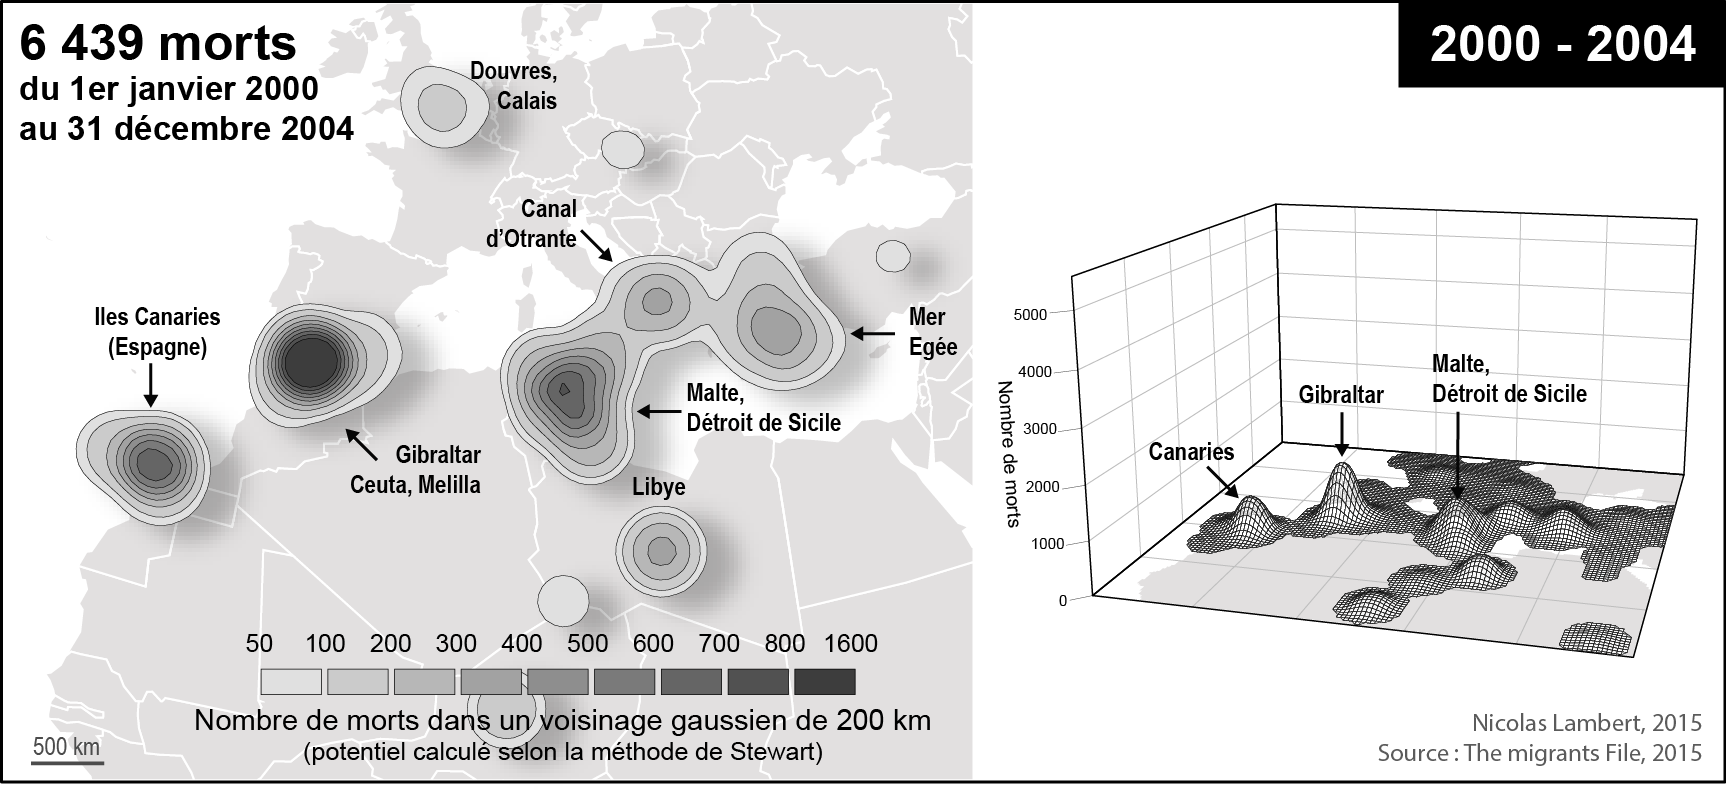
\includegraphics[width=11.5cm]{Migrants2.png}
\end{figure}

\end{frame}


% FRAME
\begin{frame}{Fields}

\textbf{Representation modes examples}

\begin{figure}
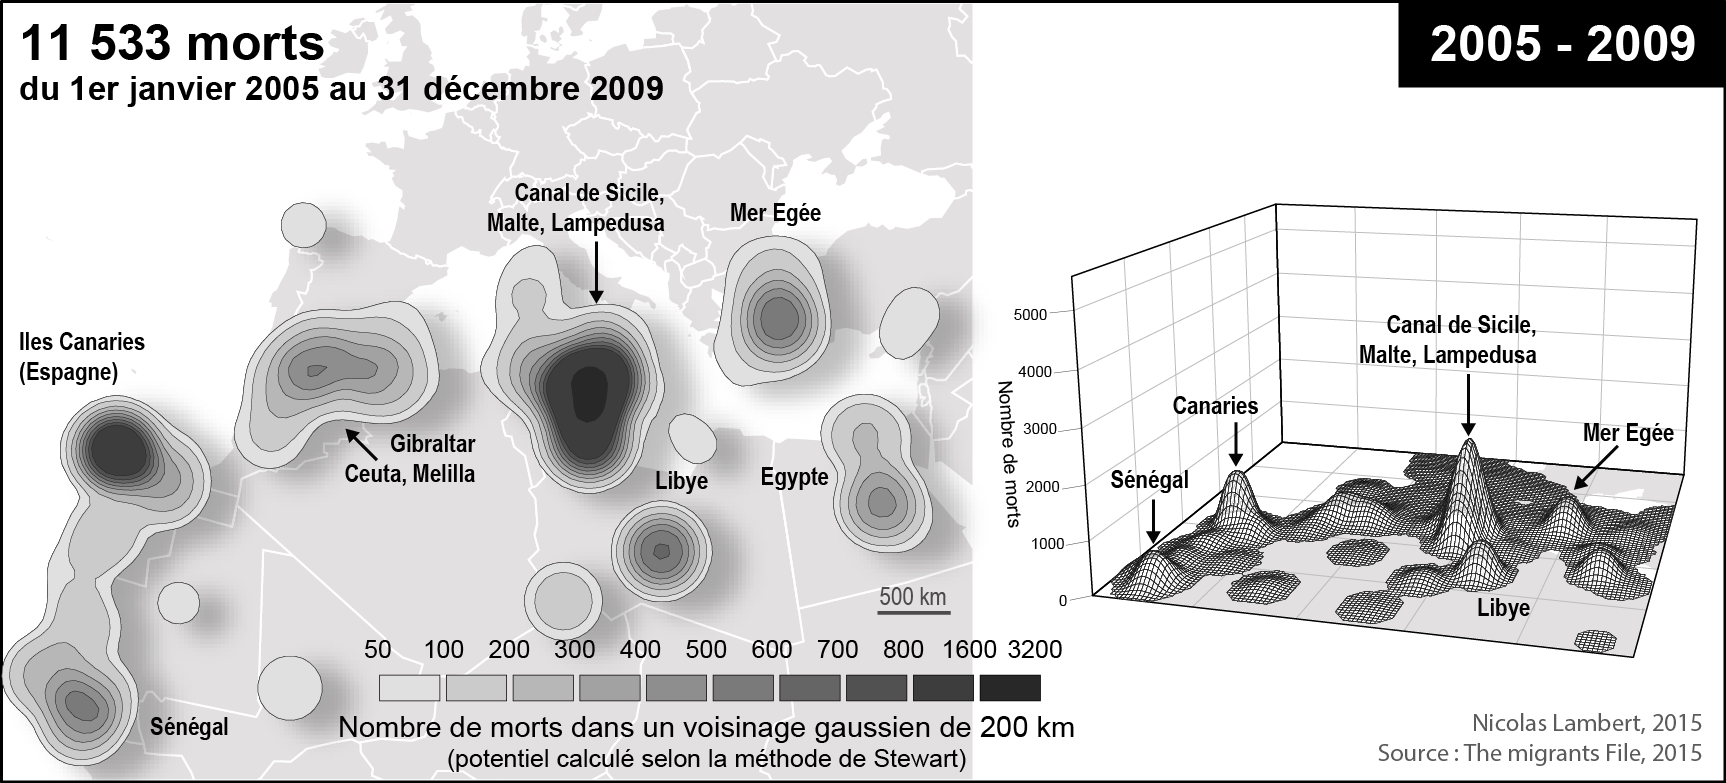
\includegraphics[width=11.5cm]{Migrants3.png}
\end{figure}

\end{frame}


% FRAME
\begin{frame}{Fields}

\textbf{Representation modes examples}

\begin{figure}
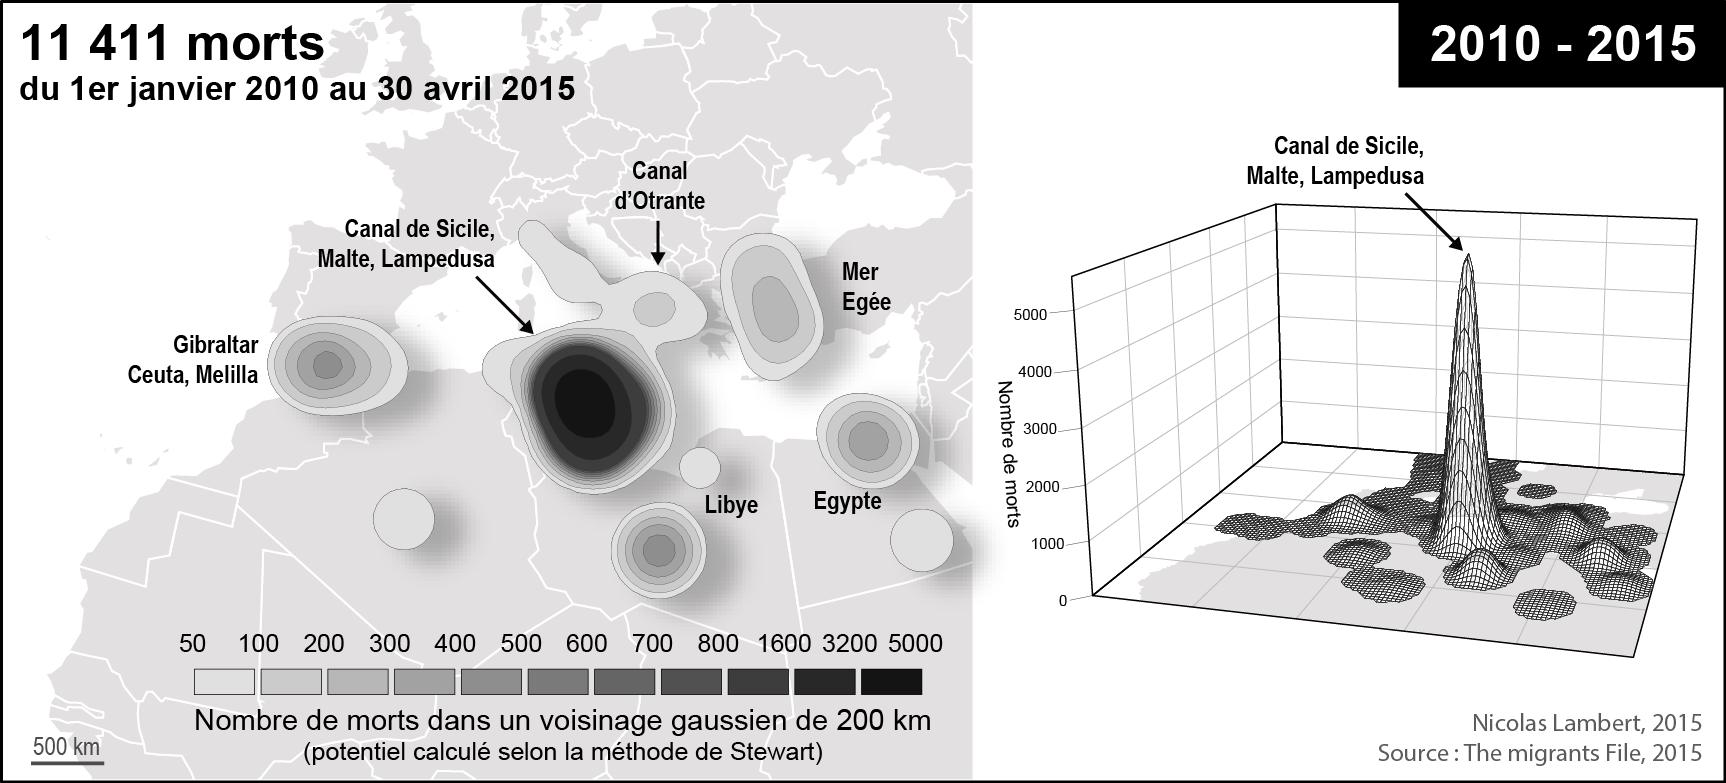
\includegraphics[width=11.5cm]{Migrants4.png}
\end{figure}

\end{frame}


% FRAME
\begin{frame}{Fields}

\begin{figure}
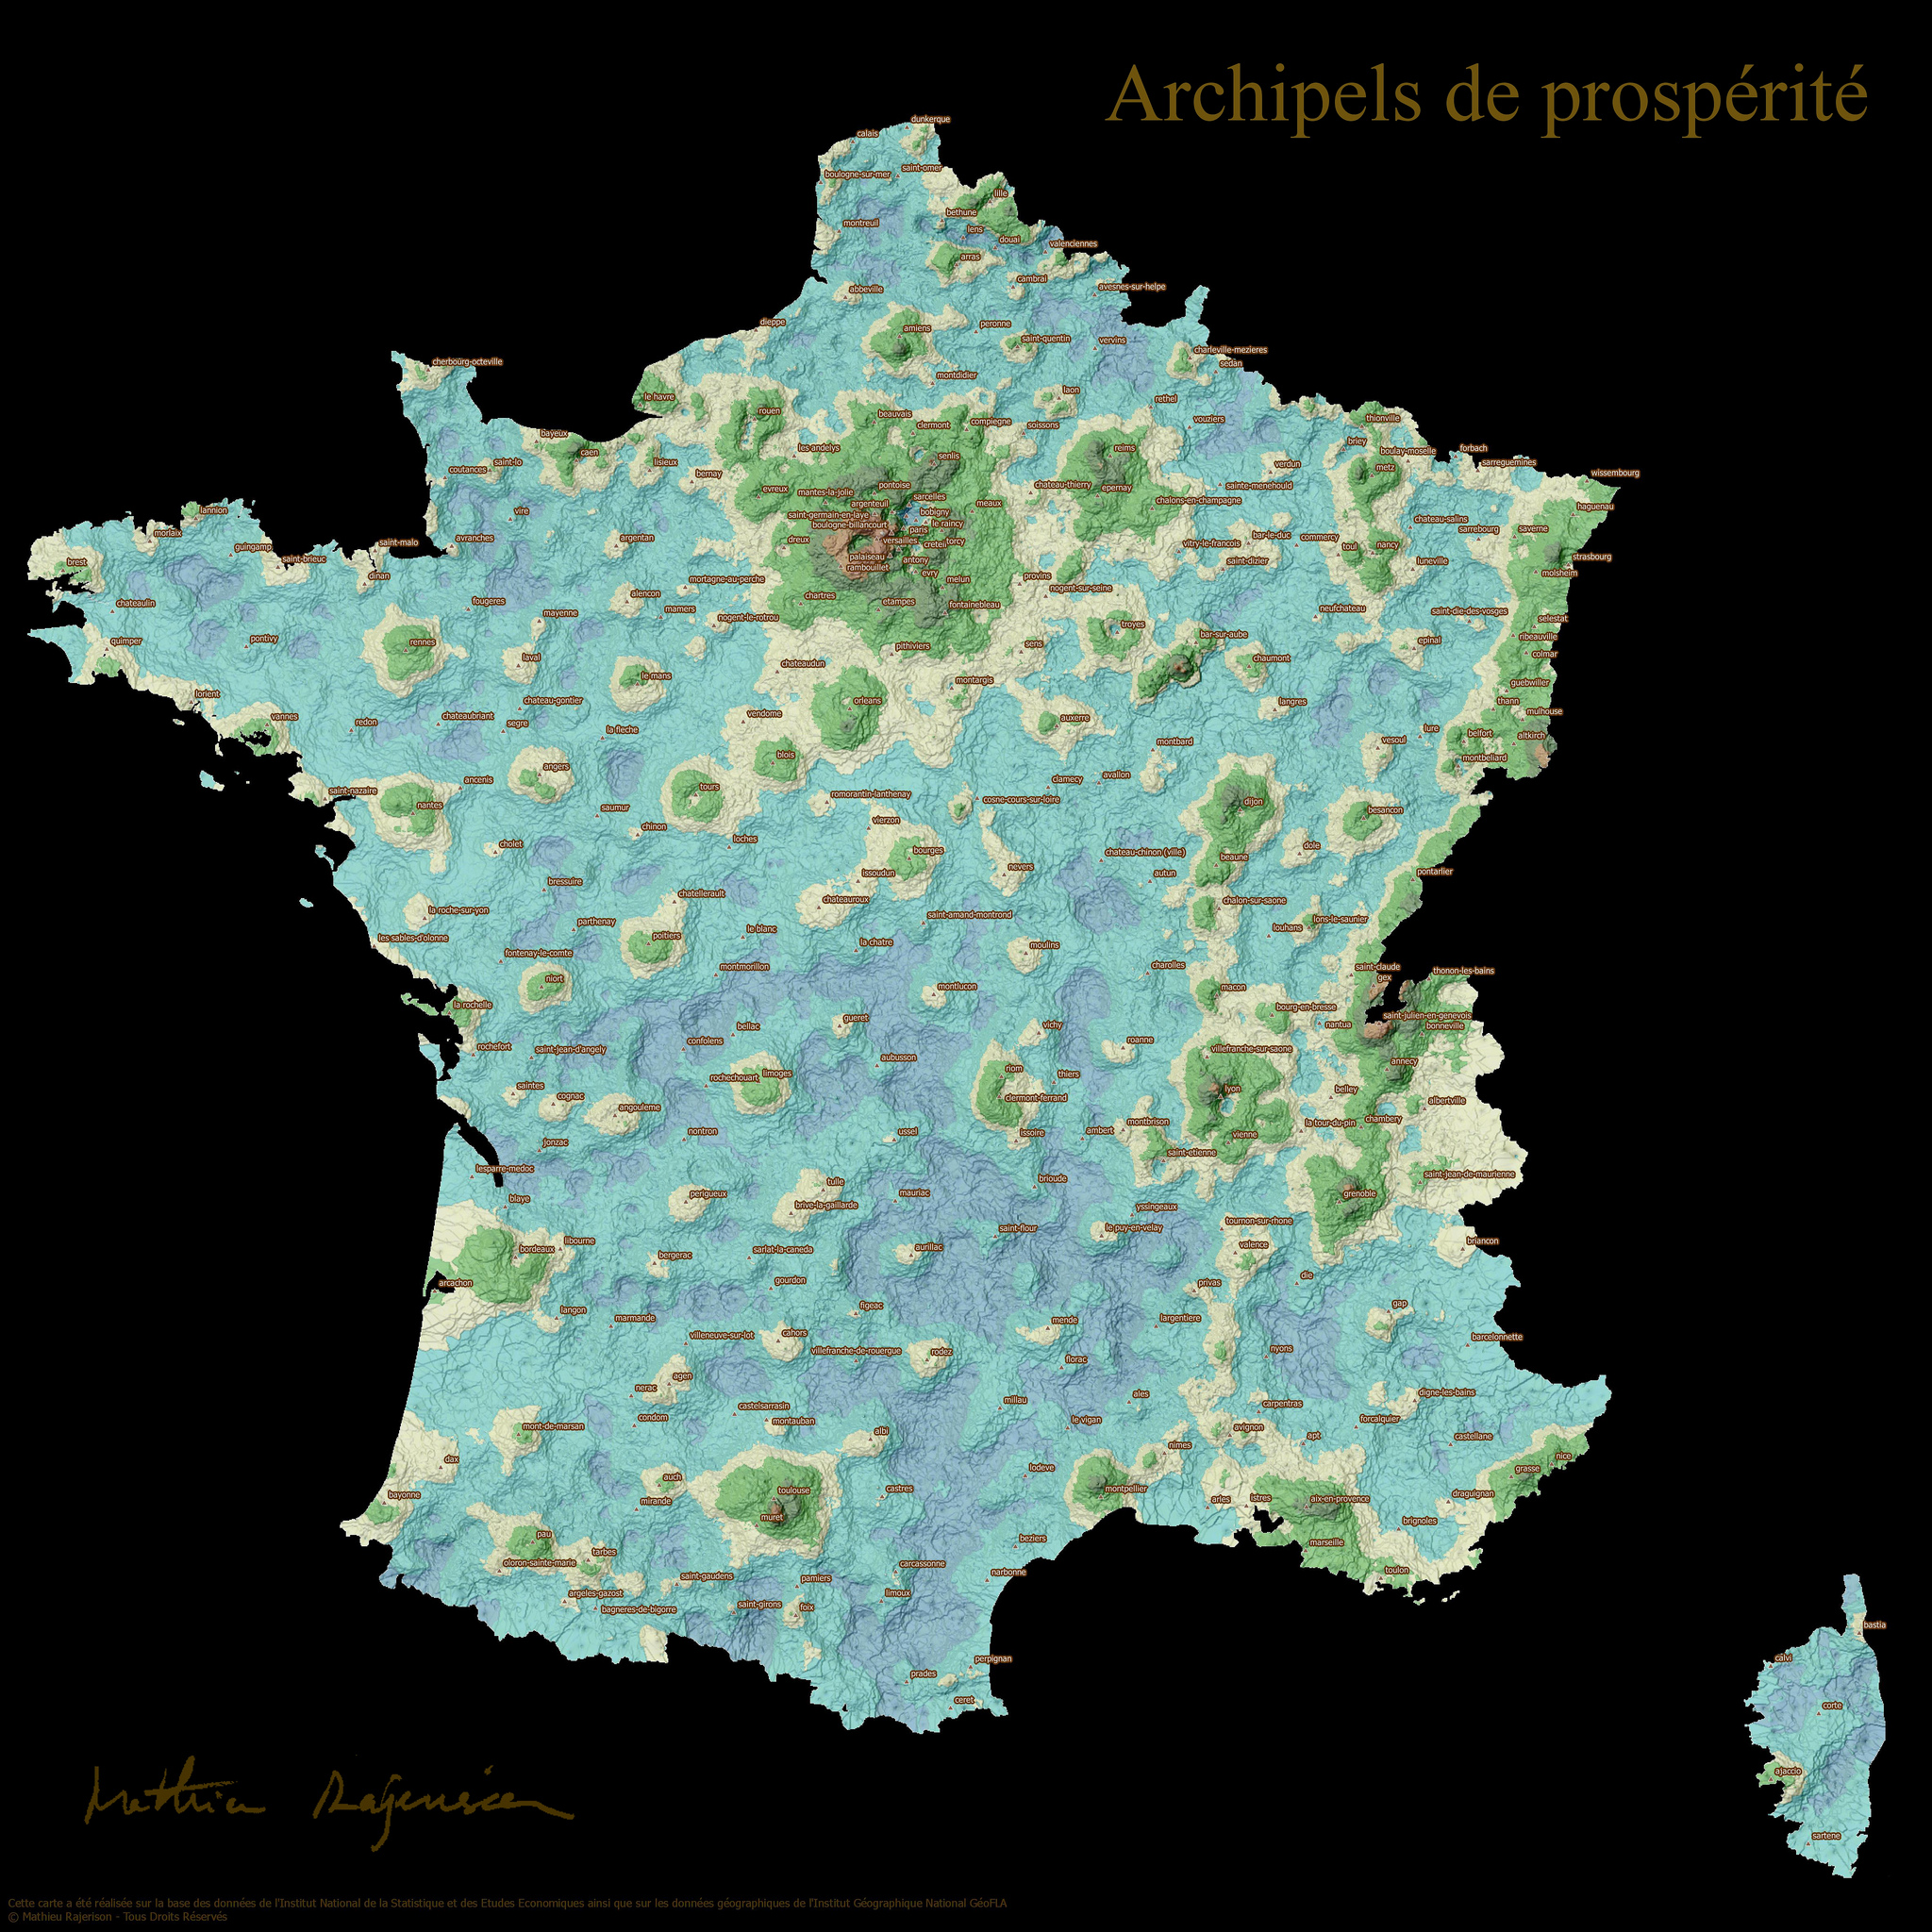
\includegraphics[width=7cm]{Rajerison_Revenu.jpg}
\end{figure}

\footnotesize
\textit{Source: Rajerison, Les archipels de la prospérité}
\normalsize

\end{frame}



% FRAME
\begin{frame}{Fields}

\begin{figure}
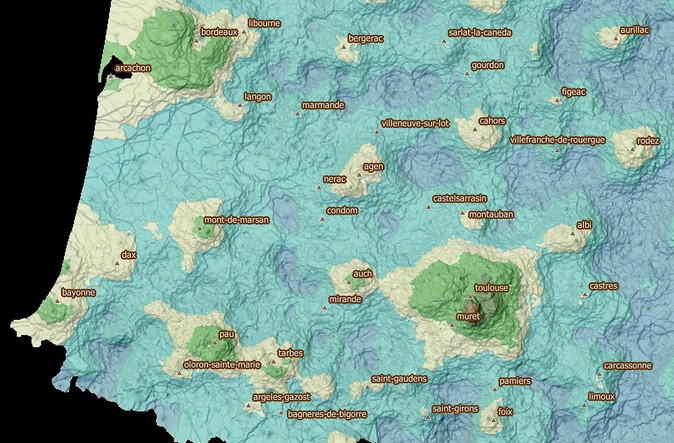
\includegraphics[width=9.5cm]{Rajerison_Zoom.jpg}
\end{figure}

\footnotesize
\textit{Source: Rajerison, Les archipels de la prospérité}
\normalsize
\end{frame}



% FRAME
\begin{frame}{Fields}
\begin{center}
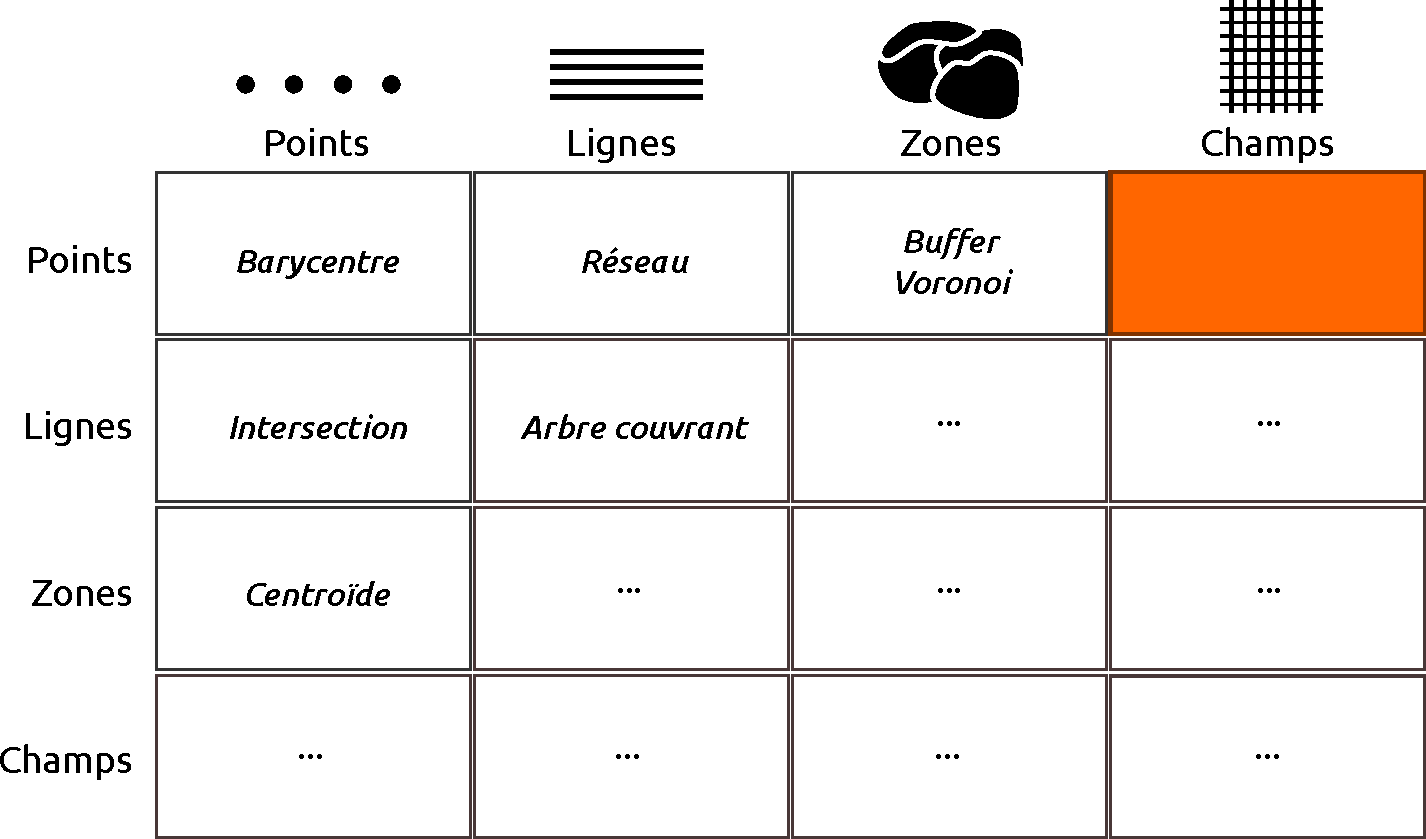
\includegraphics[width=10.5cm]{TypesObjets.pdf}
\end{center}
\end{frame}





  
  
  
\section{Simulation stochastique}

  % Définition du répertoire contenant les images
\graphicspath{{IMAGE/}}

% FRAME Intro
\begin{frame}


\includegraphics[width=12cm]{Logos.pdf}

\vfill

\begin{center}

\vspace*{1.5cm}

\LARGE
\textbf{Simulation}

\vspace*{1.5cm}
 DELHI GIS-R School


\large
9-12\up{th} April 2019

\vspace*{1.5cm}


\textbf{Hadrien Commenges \& Paul Chapron}

{\small

\vspace*{0.1cm}

\url{hadrien.commenges@univ-paris1.fr}

\url{paul.chapron@ign.fr}

}

\end{center}

\end{frame}

% FRAME
\begin{frame}{Stochastic simulation }

Stochastic simulation : data generation using \textbf{randomly drawn values}.

\begin{itemize}
\item \textbf{Monte Carlo:} generic term refering to process involving random process repetition.
\item \textbf{Bootstrap:} re-sampling methods (usually to estimate distribution) 
\item \textbf{Permutation:} reordering elements of a set   
\end{itemize}

~

\textbf{Why ? }

Most of the time:  to approach a distribution 

\begin{itemize}
\item (often) because the analytical way is hard 
\item because (sometimes) there is no analytical way 
\item because we look for robust estimation adequate to the use case data 
\end{itemize}

\end{frame}


% FRAME
\begin{frame}{Monte Carlo}

$\rightarrow$ \textbf{Example:} iterated dice rolls \\
$\rightarrow$ \textbf{Goal:} examplify the Law of Large Numbers

~

\textbf{Expected value $\mu$ of a dice roll:}

$$
\mu = \frac{1}{6} \times 1 + \frac{1}{6} \times 2 + \frac{1}{6} \times 3 + \frac{1}{6} \times 4 + \frac{1}{6} \times 5 + \frac{1}{6} \times 6
$$


$$
\mu = \frac{1+2+3+4+5+6}{6} = 3,5
$$

~

\textbf{(weak) Law of Large Numbers: }

~
\begin{center}
$\bar{X_n} \to \mu$ when $n \to \infty$
\end{center}

~

\emph{(sample average converges toward the expected value, for a sufficiently large sample)}

\end{frame}


% FRAME
\begin{frame}{Monte Carlo}
%TODO refaire figure EN
\begin{figure}
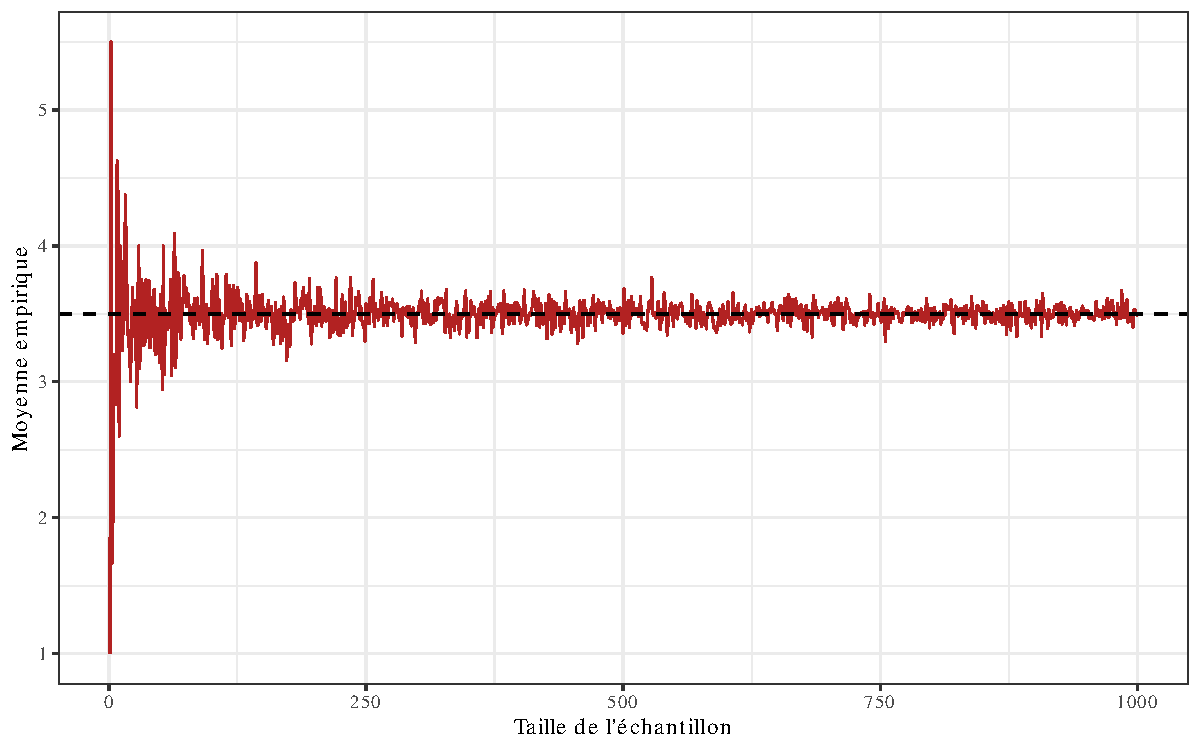
\includegraphics[width=11cm]{TirageDe.pdf}
\end{figure}

\end{frame}



% FRAME
\begin{frame}{Bootstrap}

\textbf{Classical inference:}
\begin{itemize}
  \item Goal : approach  $\mu$ and $\sigma$  \textbf{parameters} of a distribution
  \item $\bar{X}$ and $\sigma_X$ are computed on a \textbf{sample} X
  \item Sampling of X and $\bar{X}$ / $\sigma_X$ computation are repeated 
\end{itemize}

~

\textbf{Example:}
\begin{itemize}
  \item For a 12M population (people from Île-de-France).
  \item People travel daily  between  0 and 200 km.
  \item 500 samples are drawn,  100 people each.
  \item For each sample, the average travel distance ($\bar{X}$) is computed .
\end{itemize}

~

$\rightarrow$ these 500 average values form a \textit{distribution}: the \textbf{sampling distribution of the mean}

\end{frame}



% FRAME
\begin{frame}{Bootstrap}

\textbf{Sampling distribution of the mean} (500 mean values):
 
\begin{figure}
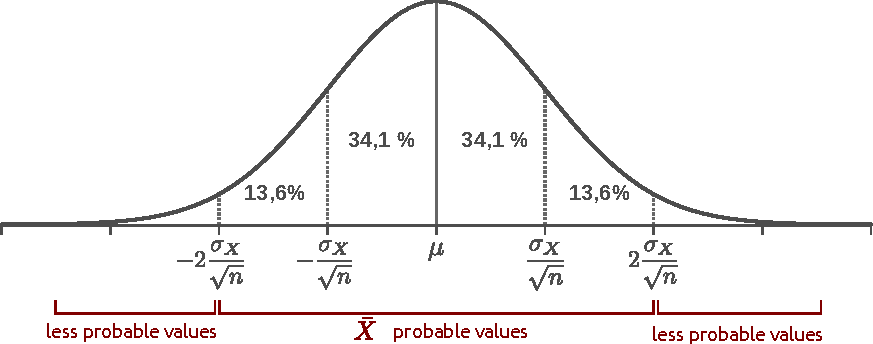
\includegraphics[width=11cm]{DensiteNormal_EN.pdf}
\end{figure}

where $\mu$ et $\sigma$ are the \textbf{parameters} --  real mean and standard deviation of the population -- and $n$ is the  \textbf{sample size}. 

~

$\rightarrow$ This is \textbf{central limit theorem} (\textbf{CLT}).

\end{frame}




% FRAME
\begin{frame}{Bootstrap}

\begin{itemize}
\item \textbf{General inference idea:} the sample (which is known) allows to approach the parameters of the population distribution (which is unknown)
\item \textbf{General bootstrap idea:} re-sampling (which is known) from the sample (which is known) give insights about what would sampling look like on the whole population.
\item \textbf{Example:} to estimate the variance of the sampling distribution , we compute the variance of the re-sampling distribution of the mean.
\end{itemize}

\end{frame}



% FRAME
\begin{frame}{Bootstrap}

\textbf{Daily travel distance for Île-de-France people}
%TODO figure EN
\begin{figure}
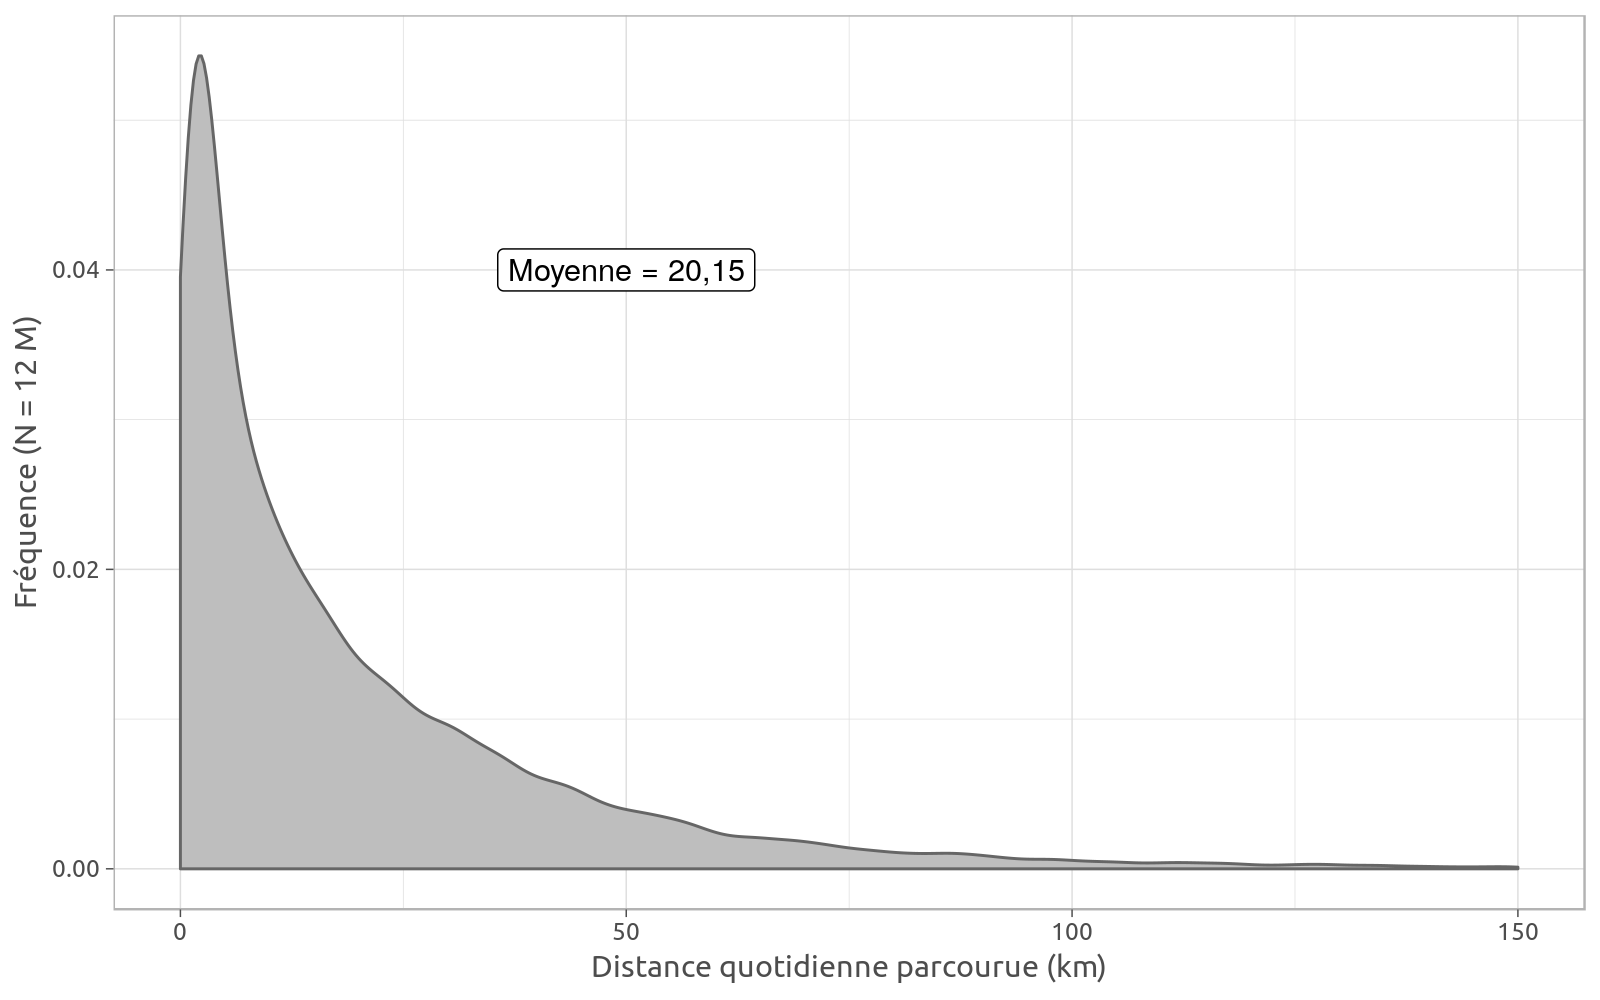
\includegraphics[width=11cm]{PopDist.png}
\end{figure}

\footnotesize
Source: Enquête Globale Transport 2010 (French transportation national census)
\normalsize

\end{frame}




% FRAME
\begin{frame}{Bootstrap}

\textbf{Sampling distribution of the mean}
%TODO figure EN

\begin{figure}
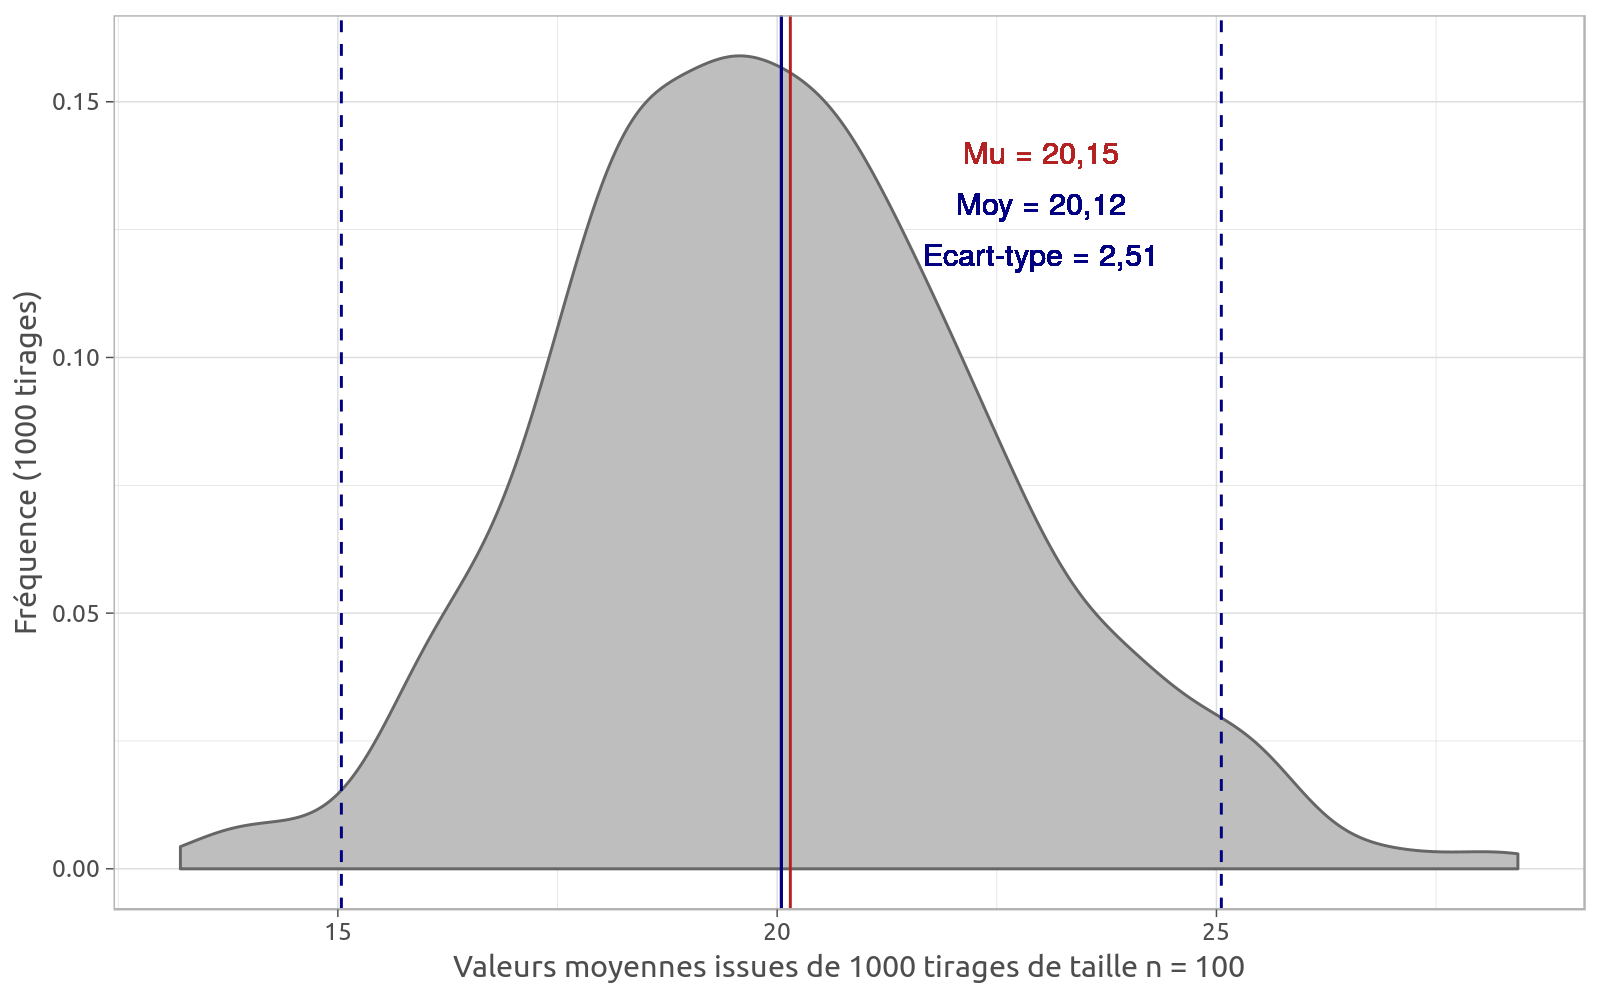
\includegraphics[width=11cm]{SampDist.png}
\end{figure}

\end{frame}


% FRAME
\begin{frame}{Bootstrap}

\textbf{Re-sampling of the mean} on a sample 

\begin{figure}
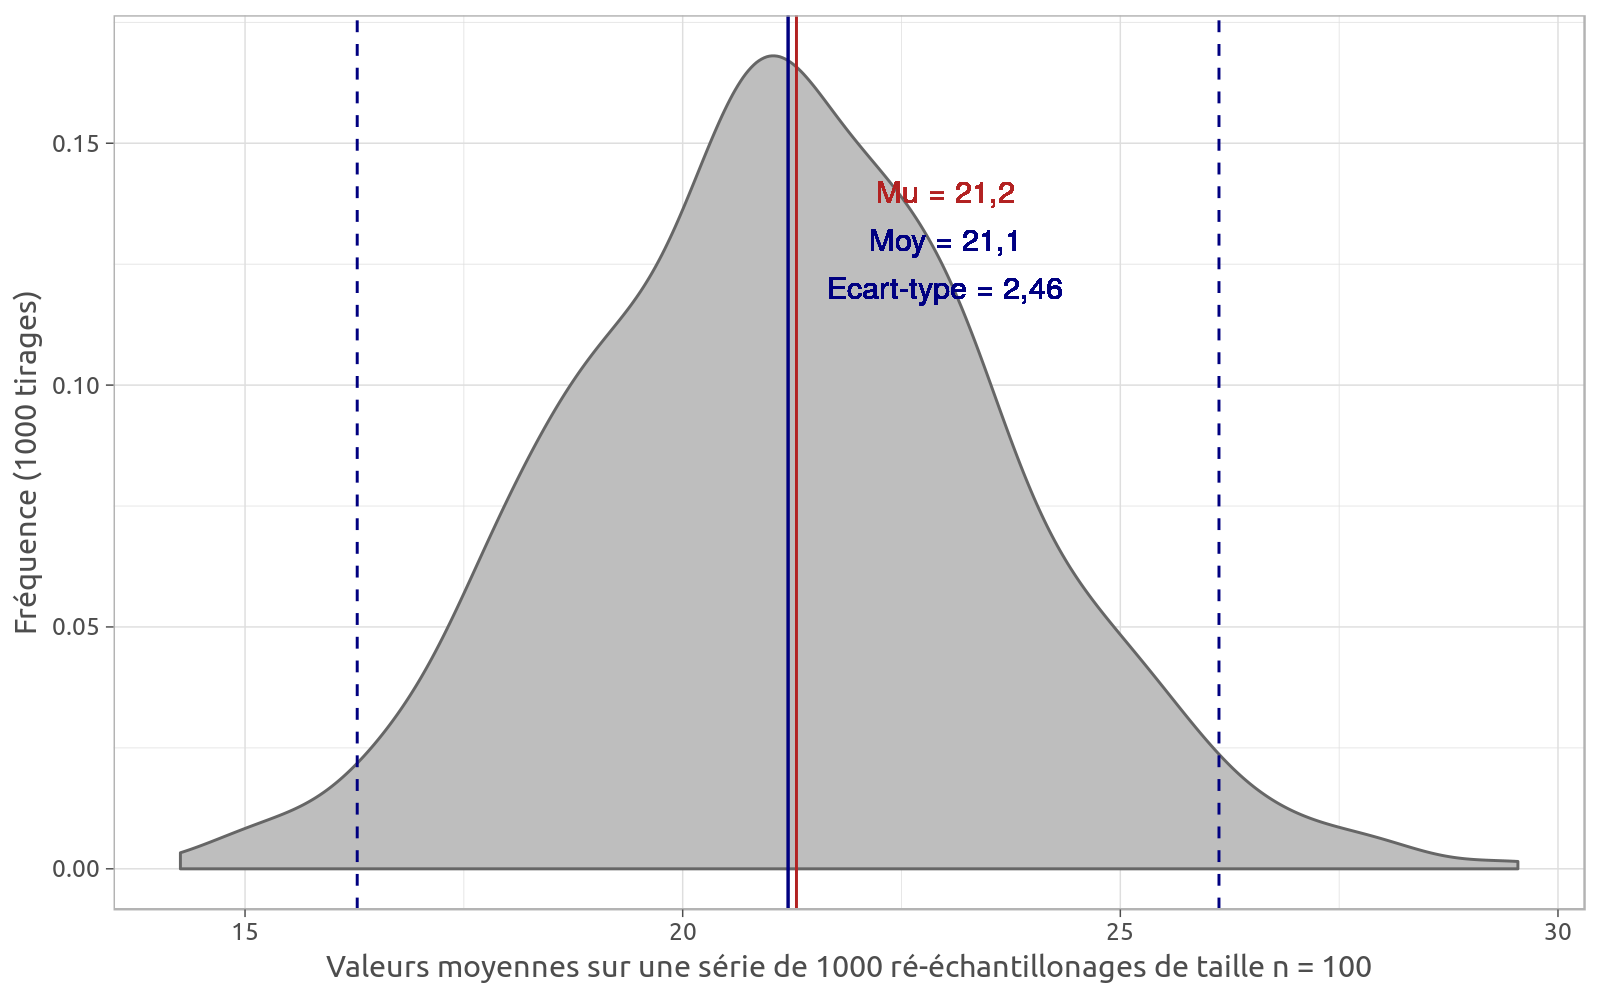
\includegraphics[width=11cm]{SampDistBoot.png}
\end{figure}

\end{frame}


% FRAME
\begin{frame}{Bootstrap}


\textbf{Power of the Bootstrap}: this technique offers

\begin{itemize}
\item compute estimates (mean, variance) without any hypothesis or \textit{a priori} knowledge on the population
\item compute estimates variability  (confidence interval) without any hypothesis or \textit{a priori} knowledge on the population (\textit{distribution-free confidence intervals})
\item assess the stability of some model results  (\textit{cross-validation})
\end{itemize}

\end{frame}




  
\section{Density}

 % Définition du répertoire contenant les images
\graphicspath{{IMAGE/}}

% FRAME Intro
\begin{frame}


\includegraphics[width=12cm]{Logos.pdf}

\vfill

\begin{center}

\vspace*{1.5cm}

\LARGE
\textbf{Density}

\vspace*{1.5cm}
 DELHI GIS-R School


\large
9-12\up{th} April 2019

\vspace*{1.5cm}


\textbf{Hadrien Commenges \& Paul Chapron}

{\small

\vspace*{0.1cm}

\url{hadrien.commenges@univ-paris1.fr}

\url{paul.chapron@ign.fr}
}

\end{center}

\end{frame}

% FRAME
\begin{frame}{Use case}

\begin{block}{Density}
Density is a \textbf{spatial variable} depicting the \textbf{spatial variation} of some observations (concentration and dispersion) in 1, 2 or $n$ dimensions. 
\end{block}

\begin{itemize}
\item Mass / Volume ratio (volumetric mass), mass per volume unit, sometimes ratio between an object volumetric mass and a reference volumetric mass. 
\item Ratio between a \textbf{count}  and its \textbf{extent}: a variable's density (1D), population density (2D, so \textbf{spatial extent}), etc.
\end{itemize}

~

\textbf{What kind of geographical information is concerned ?}

$\rightarrow$ \textit{TYPE 1 - Geographical Objects}

$\rightarrow$ \textit{TYPE 2 - Occurrences}

\end{frame}


% FRAME
\begin{frame}{Goals}

\textbf{Main uses:}

\begin{enumerate}
  \item Describe a point pattern 
  \item Estimate the probability of an event to occur at a given point
  \item Estimate the probability that a spatial distribution of events is random.
\end{enumerate}

\end{frame}


% FRAME
\begin{frame}{Spatial distribution parameters}

\textbf{Centrality} and \textbf{dispersion} can be computed in a 1, 2 2 or $n$ dimensions space. 

~

Current analysis of these parameters:

\begin{itemize}
\item Description of a distribution: mean and standard deviation
\item Evolution of these parameters over time
\item Parameters weight
\end{itemize}

\end{frame}


% FRAME
\begin{frame}{Spatial distribution parameters}

2-Dimensions \textbf{mean}  : \textbf{barycenter} (or \textbf{balancing point } ).

$$
x_g = \frac{\sum_{i=1}^n w_i x_i}{\sum_{i=1}^n w_i} ~~~~~~~~~~~~~~~ y_g = \frac{\sum_{i=1}^n w_i y_i}{\sum_{i=1}^n w_i}
$$

~

~

$\rightarrow$ weights $w_i$ might be constant or varying, depicting localized stocks variations.

\end{frame}



% FRAME
\begin{frame}{Spatial distribution parameters}

2-Dimensions \textbf{variance} $\approx$ \textbf{inertia}.

\begin{figure}
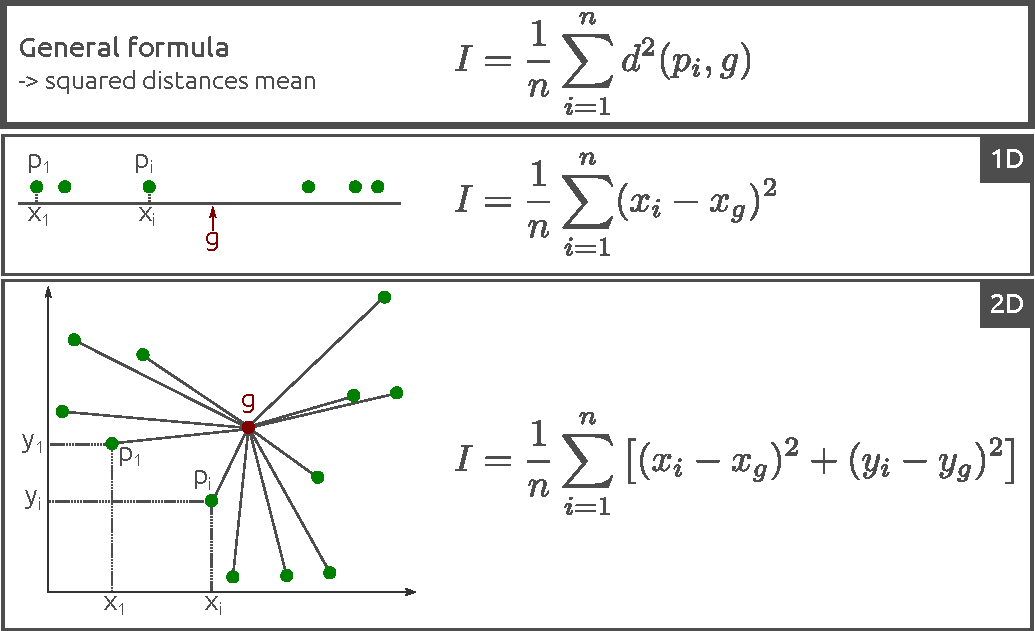
\includegraphics[width=11cm]{Inertie_EN.pdf}
\end{figure}


\end{frame}

% FRAME
\begin{frame}{Spatial distribution parameters}

\begin{figure}
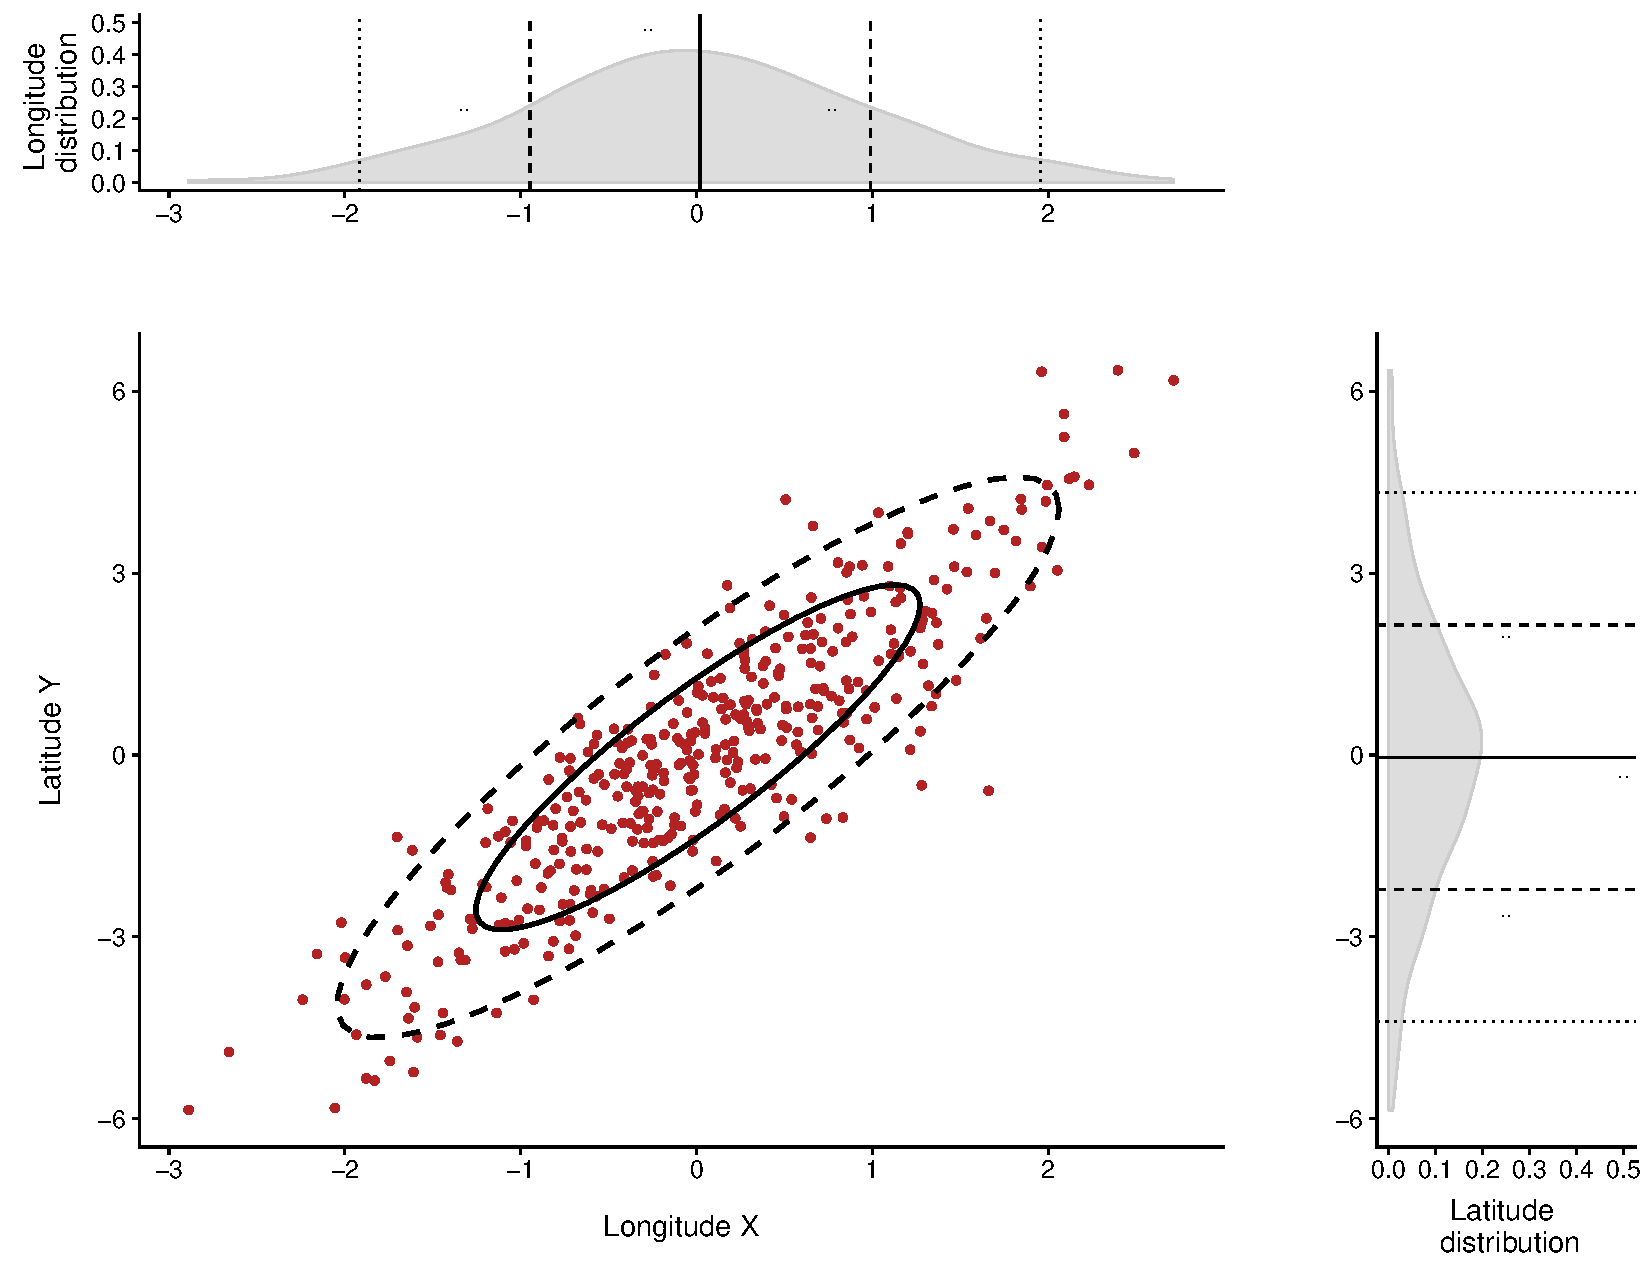
\includegraphics[width=9cm]{Ellipsis_dev_EN.pdf}
\end{figure}

\end{frame}


% FRAME
\begin{frame}{Spatial distribution parameters}

\begin{figure}
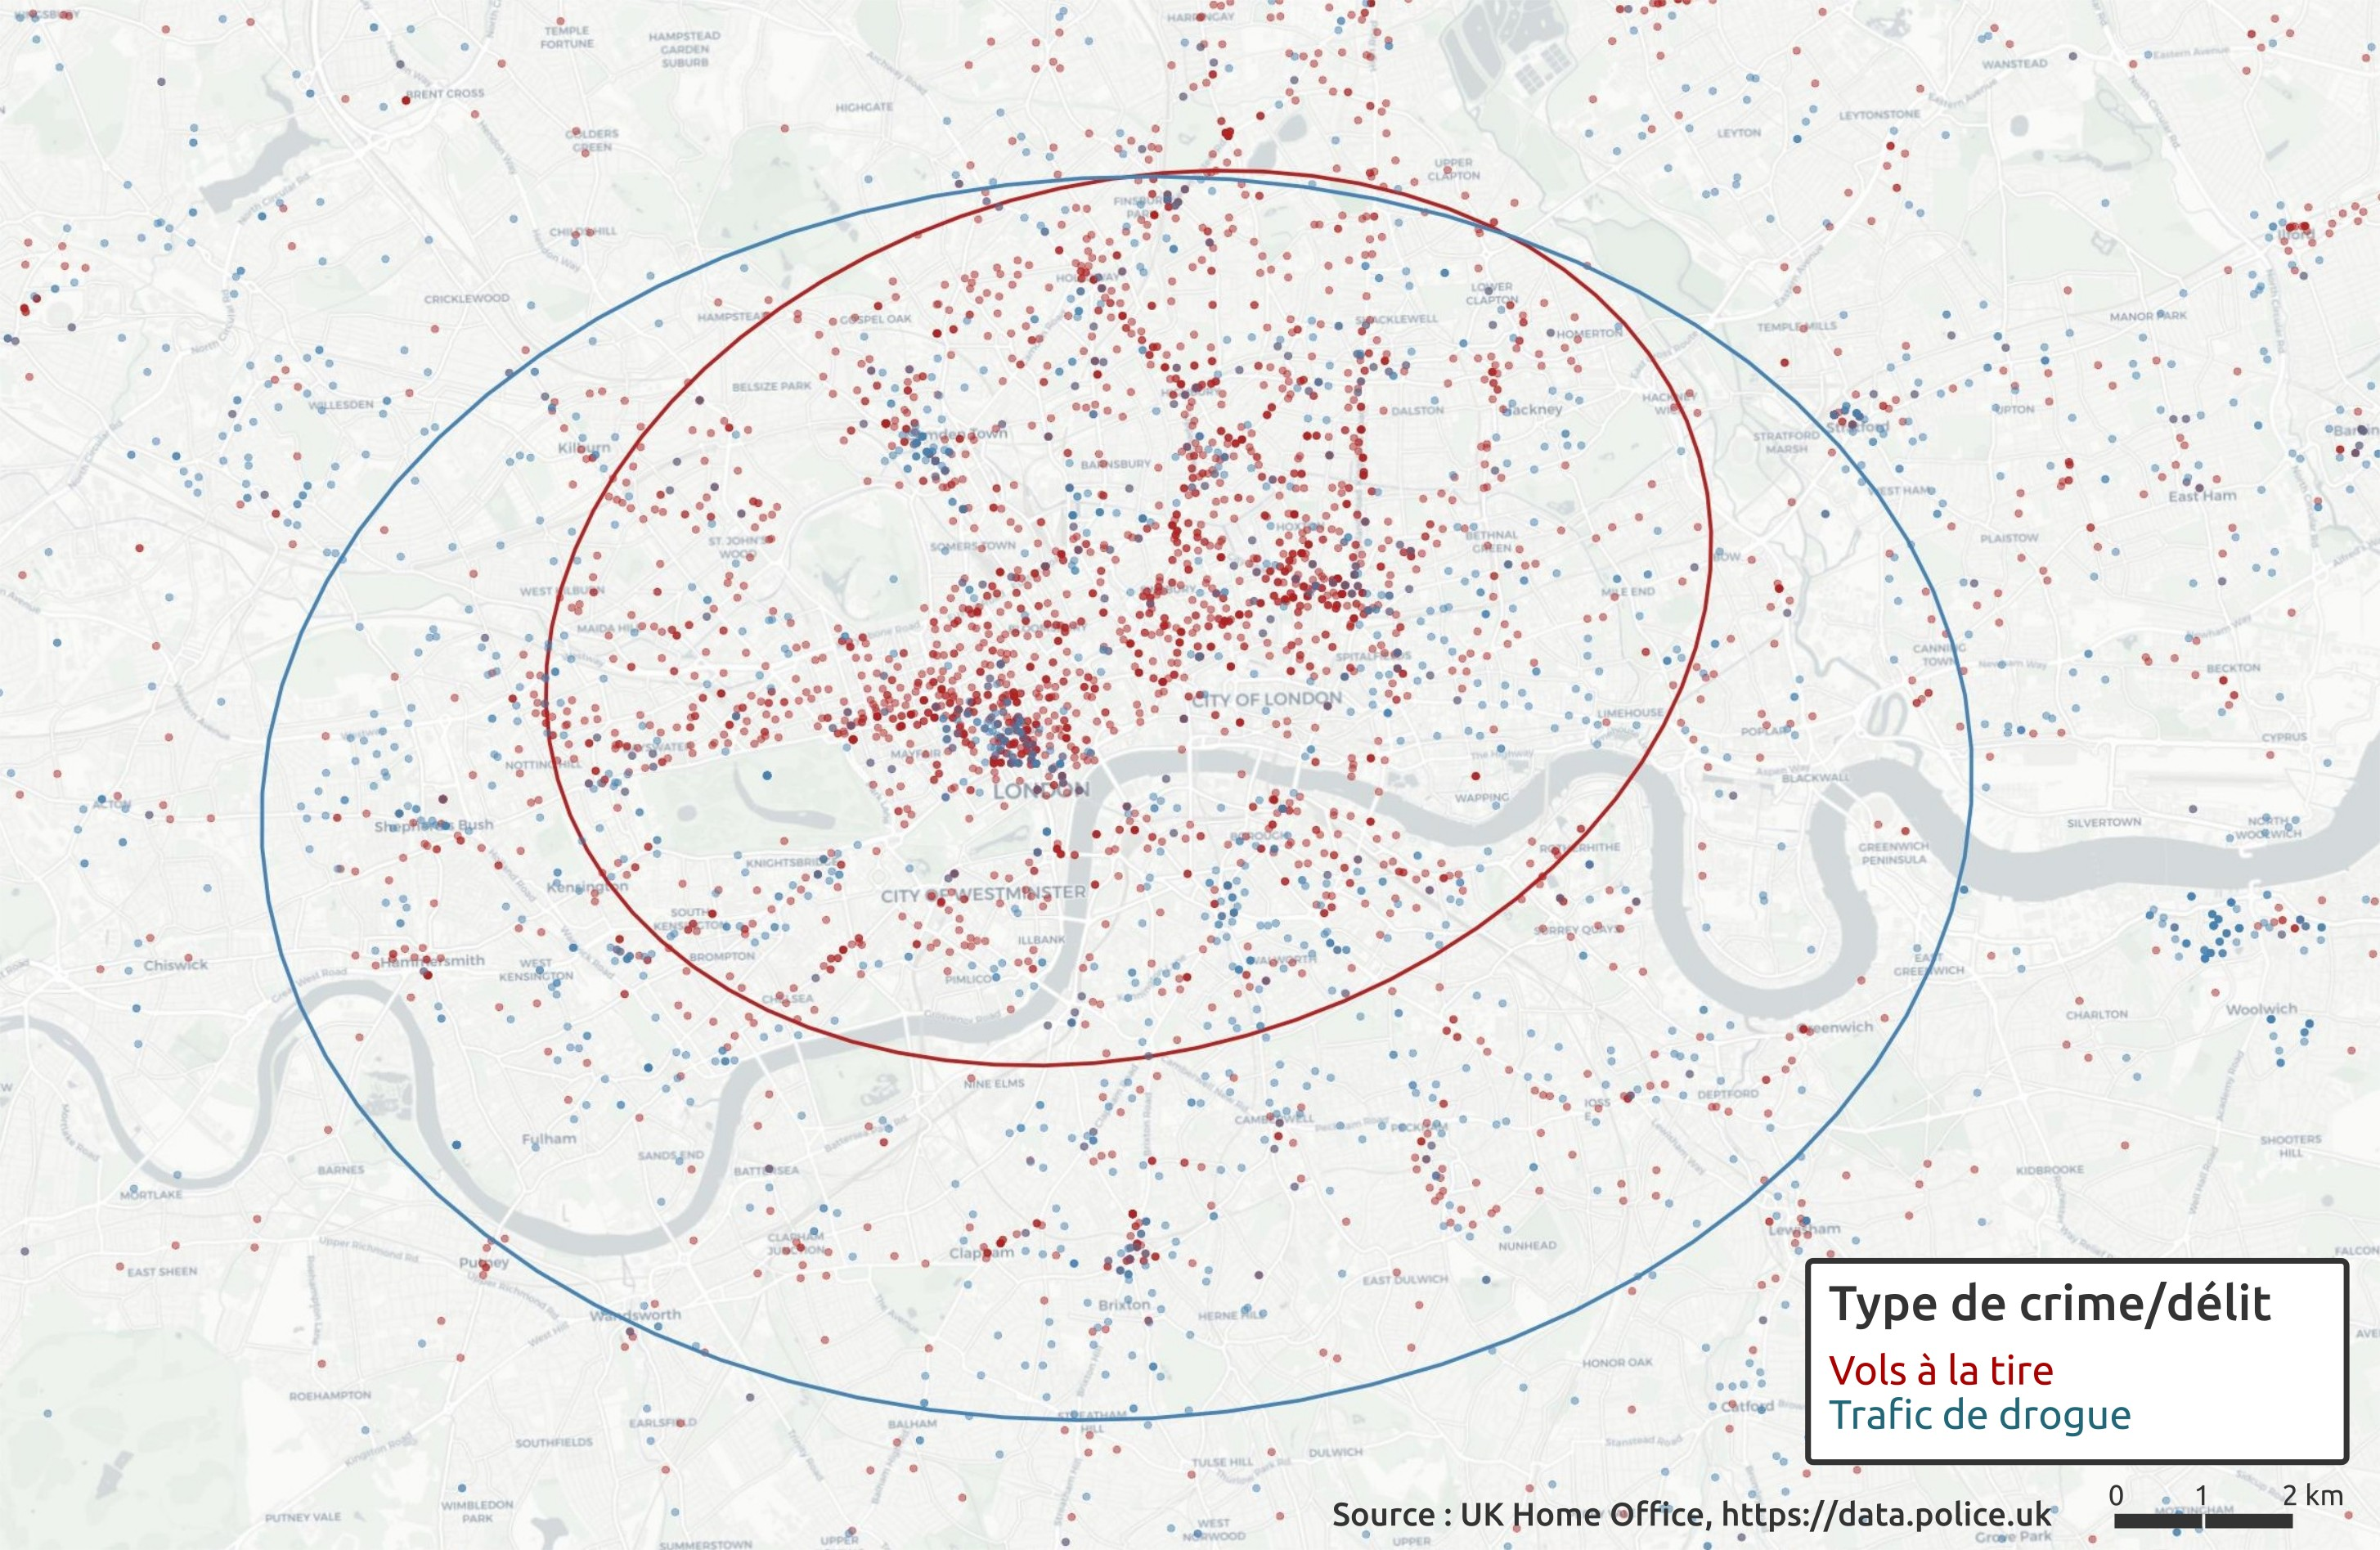
\includegraphics[width=12cm]{Crimes.jpg}
\end{figure}

\end{frame}



% FRAME
\begin{frame}{Spatial distribution parameters}

\begin{figure}
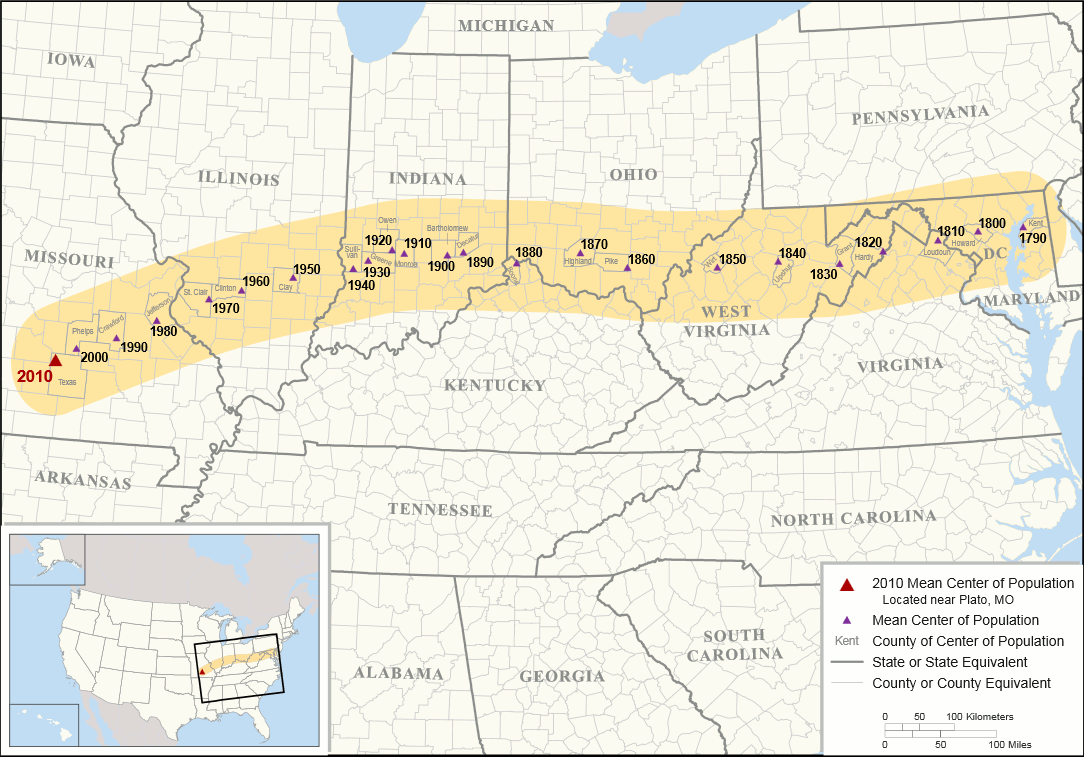
\includegraphics[width=10cm]{Centerpop.png}
\end{figure}

\footnotesize
Source: US Census, \url{https://www.census.gov/geo/reference/centersofpop.html}
\normalsize

\end{frame}


% FRAME
\begin{frame}{1D distribution graph (discrete)}

\textbf{Histogram}

~ 

\begin{figure}
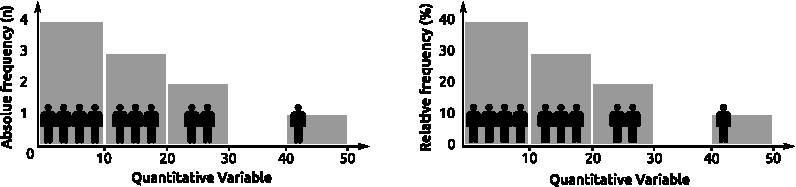
\includegraphics[width=12cm]{Histogramme_EN.pdf}
\end{figure}

$\rightarrow$ histogram estimated density is \textbf{discrete} by construction.

\end{frame}



% FRAME
\begin{frame}{Distribution graph (Parzen)}

\textbf{Histogram generalization: Parzen window}

~ 

\begin{figure}
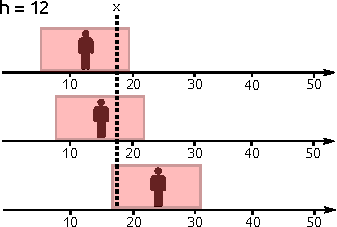
\includegraphics[width=6cm]{HistogrammeParzen.pdf}
\end{figure}

$$ D(x) = \frac{1}{3 \times 12} (1 + 1 + 1) = \frac{1}{12}$$

\end{frame}


% FRAME
\begin{frame}{Distribution graph (continuous)}

\textbf{Parzen Generalization: Gaussian Kernel}

\begin{figure}
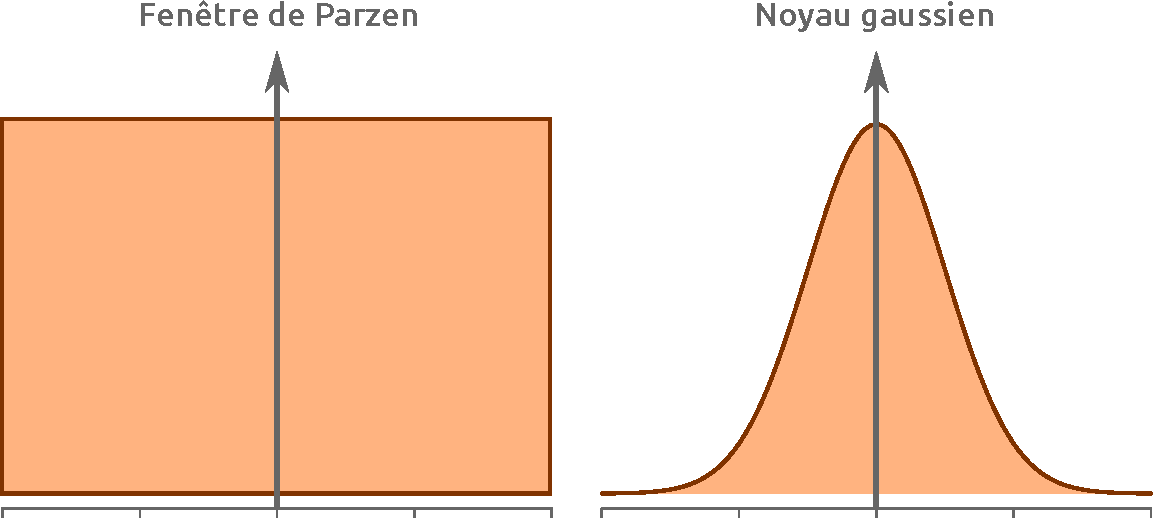
\includegraphics[width=10cm]{Gauss.pdf}
\end{figure}

\end{frame}





\begin{frame}{1D distribution graph (continuous)}

\textbf{Kernel Density Estimate}

General idea: density for a value $x$ is estimated by the proportion of observation \textit{near $x$}  

«Near» is defined by a certain window described by a \textbf{kernel function} (usually gaussian).

Contribution of each observation within the window is given by kernel function value taken for each $x$. $implies$ smoothing


\begin{figure}
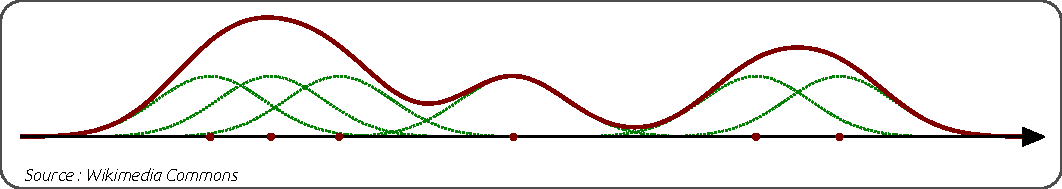
\includegraphics[width=12cm]{KDE.pdf}
\end{figure}

«Close observations contribute strongly, far ones contribute slightly »

~

\textit{Kernel Density Estimator}) may be applied in 1 to $n$ dimensions. 
For spatial analysis, we use the \textbf{2D} version.

\end{frame}


% FRAME
\begin{frame}{Distribution mapping}

Density obtained by (KDE) in \textbf{2 Dimensions}.

\begin{figure}
  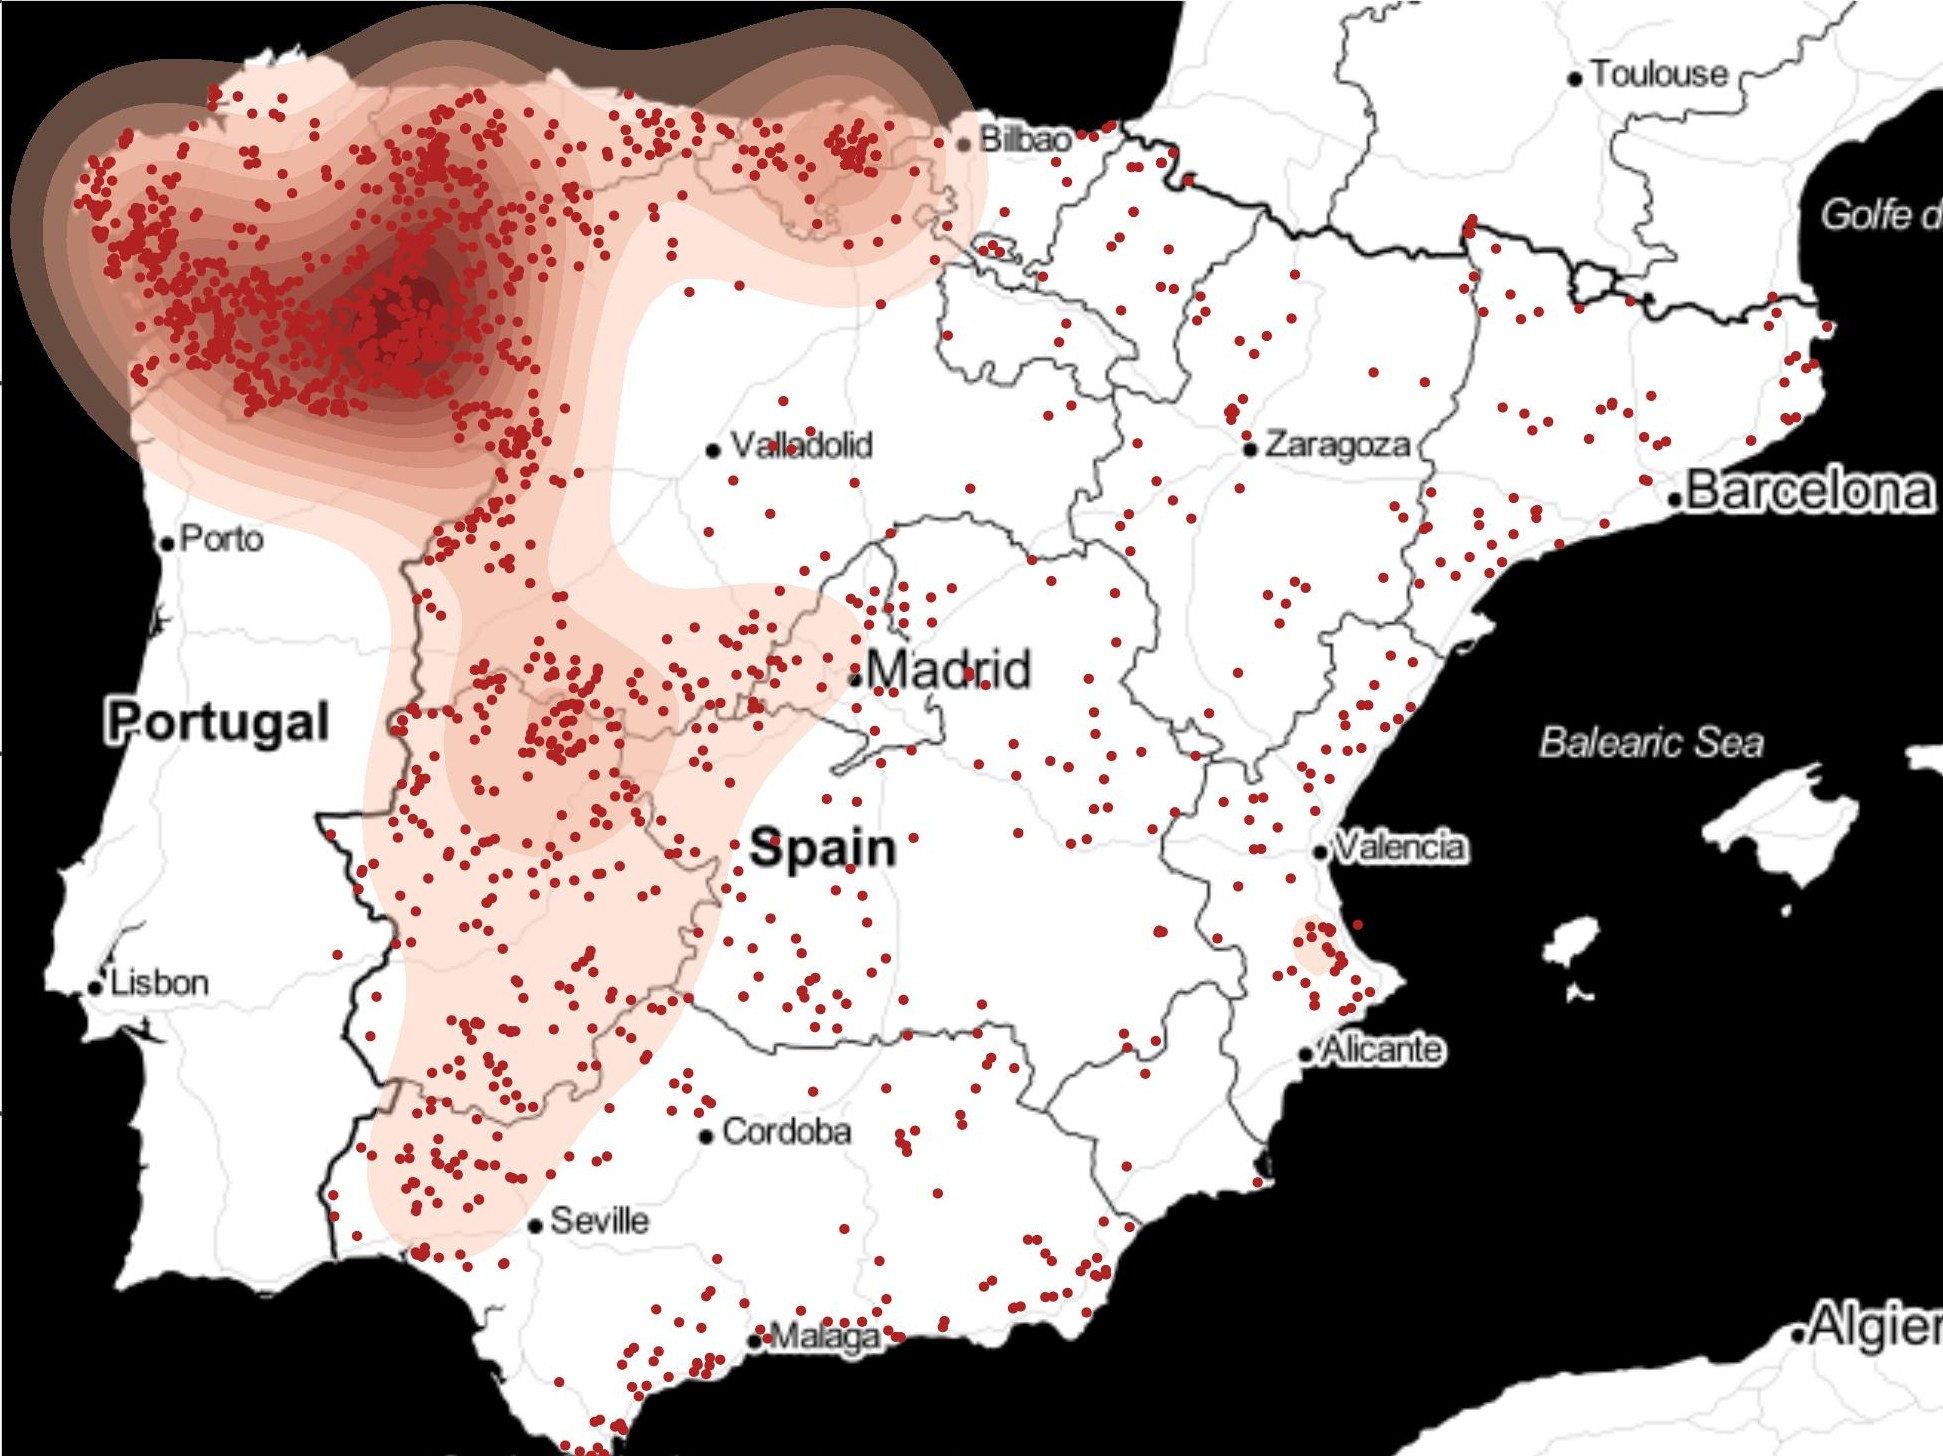
\includegraphics[width=8cm]{Incendies.jpg}
\end{figure}

\end{frame}


% FRAME
\begin{frame}{Distribution testing}

\textbf{May this distribution have been generated by a stochastic process ?}

\begin{figure}
  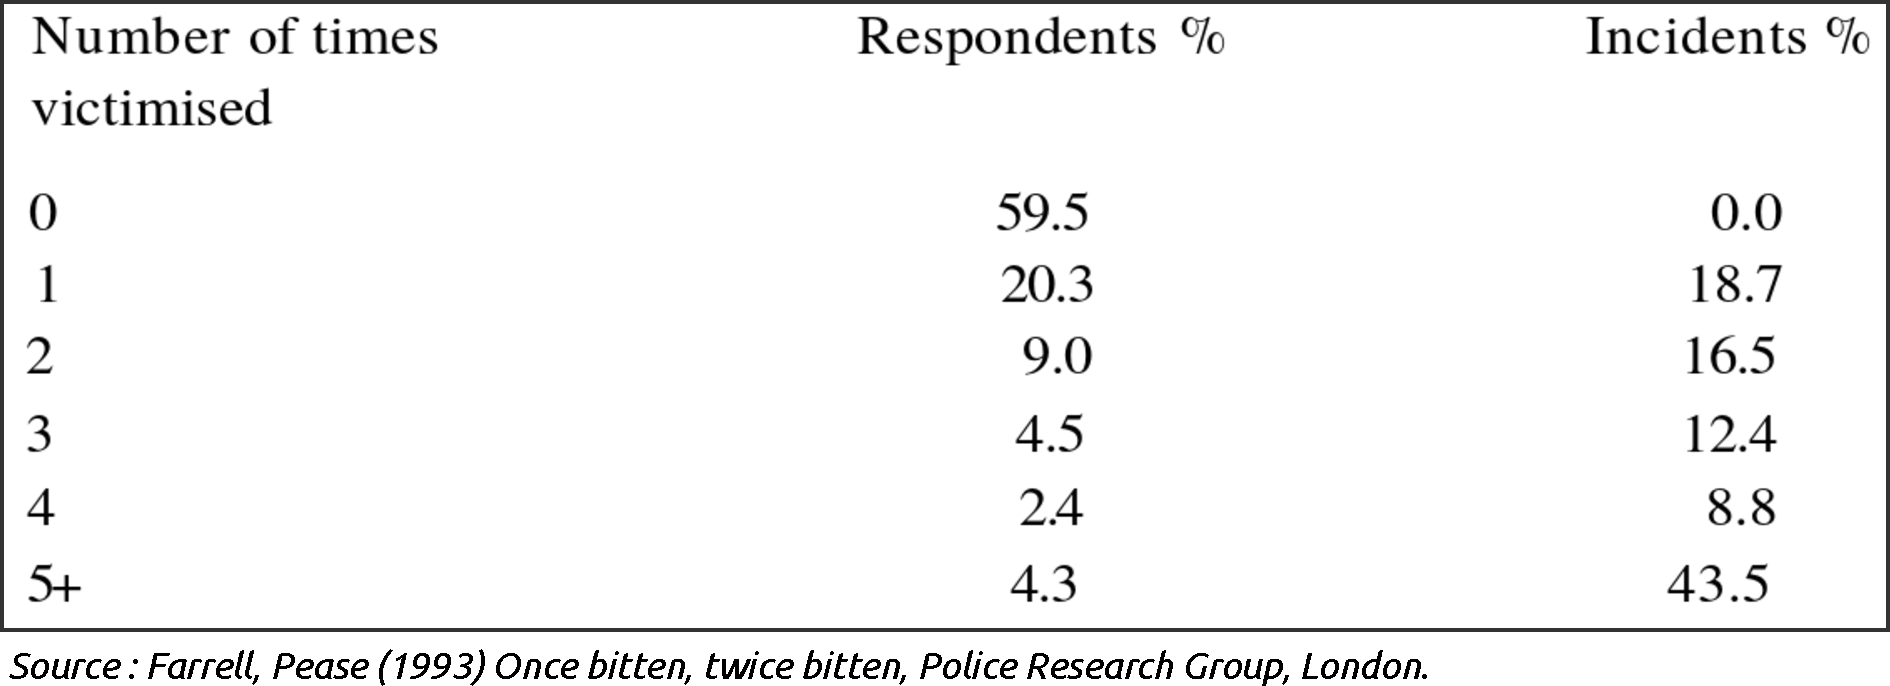
\includegraphics[width=11cm]{CrimeConcentration.pdf}
\end{figure}

\end{frame}


% FRAME
\begin{frame}{Distribution testing}
\textbf{May this distribution have been generated by a stochastic process ?}

\begin{figure}
  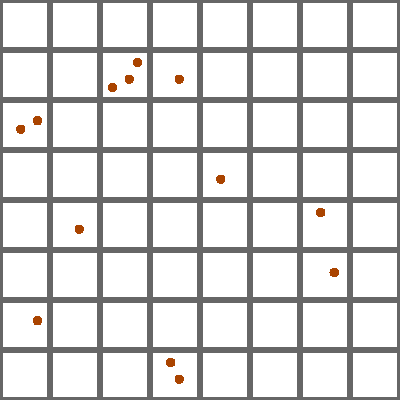
\includegraphics[width=6.5cm]{ExPoisson.pdf}
\end{figure}

\end{frame}


% FRAME
\begin{frame}{Distribution testing}

\textbf{May this distribution have been generated by a stochastic process ?}

\begin{figure}
  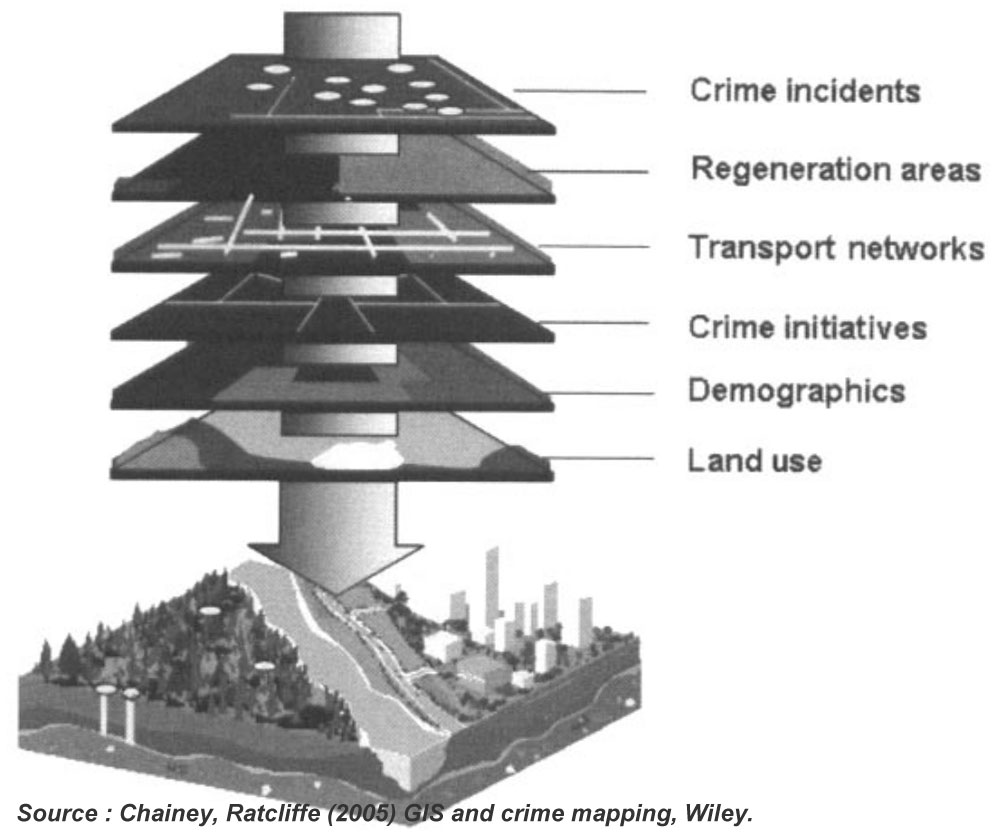
\includegraphics[width=7cm]{Chainey.jpg}
\end{figure}

\end{frame}


% FRAME
\begin{frame}{Poisson distribution}

Poisson's distribution $\lambda$ parameter is both the \textbf{mean} and the \textbf{variance} of the distribution.

\begin{equation}
\nonumber
P(X = k) = \frac{\lambda^k e^{-\lambda}}{k!}
\end{equation}


\begin{figure}
  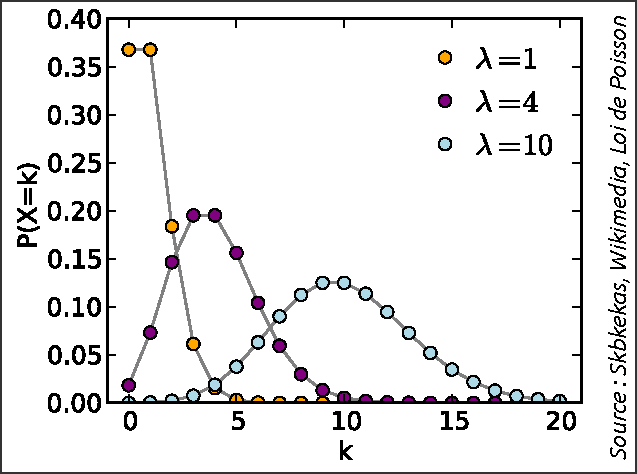
\includegraphics[width=7cm]{Poisson.pdf}
\end{figure}

\end{frame}



% FRAME
\begin{frame}{Poisson spatial distribution}

A \textbf{Poisson spatial process} is a \textbf{spatial stochastic process}, sometimes labelled as :

\begin{itemize}
  \item \textit{spatial Poisson process}
  \item \textit{homogeneous Poisson process}
  \item \textit{complete spatial randomness} (CSR)
\end{itemize}

Given a partitioned space $Z$, the probability of a given number of occurences in a zone $z$ is modeled by a Poisson distribution whose mean is  $\lambda \times area(z)$.

\end{frame}


% FRAME
\begin{frame}{Dispersion index}

\textbf{VMR} \textit{Variance-to-Mean Ratio} $=\frac{\mu}{\sigma^2}$

\begin{itemize}
\item Construct a regular grid 
\item Count occurrences
\item Compute variance,  mean and VMR
\end{itemize}

~

\textbf{VMR intrepretation}

\begin{itemize}
  \item VMR = 0 : not dispersed 
  \item VMR = 1 : may have been obtained by a Poisson process
  \item VMR < 1 : uniform / periodic
  \item VMR > 1 : concentrated / clusters
\end{itemize}

\end{frame}


% FRAME
\begin{frame}{Dispersion index}

\begin{figure}
  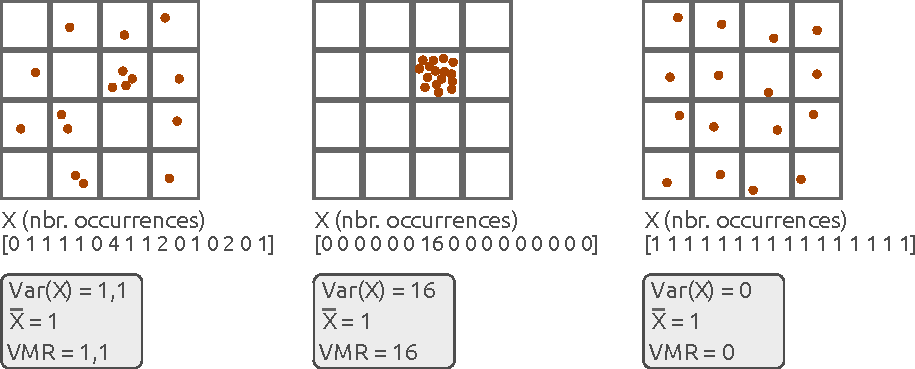
\includegraphics[width=12cm]{VMR.pdf}
\end{figure}

$\rightarrow$ \textbf{test:}  does VMR differs from 1 significantly ? (Student)

\end{frame}


% FRAME
\begin{frame}{Quadrat methods}

« A spatial $\chi^2$»

\begin{itemize}
  \item Construct a regulard grid (quadrats): observed distribution 
  \item Theoretical distribution (null model) is given by a spatial Poisson process.
  \item Contingency tables with  observed and expected occurrences
\end{itemize}

$\rightarrow$ \textbf{test:} Observations differ significantly from expected values ?  ($\chi^2$ test)

\end{frame}



\section{Interaction}

% Définition du répertoire contenant les images
\graphicspath{{IMAGE/}}

% FRAME Intro
\begin{frame}


\includegraphics[width=12cm]{Logos.pdf}

\vfill

\begin{center}

\vspace*{1.5cm}

\LARGE
\textbf{Interactions \& Networks}

\vspace*{1.5cm}
 DELHI GIS-R School


\large
9-12\up{th} April 2019

\vspace*{1.5cm}


\textbf{Hadrien Commenges \& Paul Chapron}

{\small

\vspace*{0.1cm}

\url{hadrien.commenges@univ-paris1.fr}

\url{paul.chapron@ign.fr}
}

\end{center}

\end{frame}



% FRAME
\begin{frame}{Use case}

\begin{block}{Interaction}
Relationship among objects.  An interaction may be unidirectional, bi-directional or multi-directional . 
If the entities are spatial objects, interaction always integrate a spatial dimension.
\end{block}

~

Relationships come in many forms

\begin{itemize}
\item Environment: migratory birds, climate refugees, home-to-work commutes, etc.
\item «Material realm»: commercial exchanges, percolation,   
\item «Immaterial realm» : twin-towns, Facebook friendship, co-authorship, etc.
\end{itemize}


~

\textbf{What kind of geographical information is concerned ?}



$\rightarrow$ \textit{TYPE 1 - Geographical Objects}

$\rightarrow$ \textit{TYPE 2 - Occurrences}



\end{frame}



% FRAME
\begin{frame}{Relations Modeling}

Interacting systems can be represented  by the \textbf{relations} between constitutive \textbf{entities} , either as an \textbf{(adjacency) matrix} or as a \textbf{list of links}, weighted or not. (cf Graphs)

%TODO figure EN 
\begin{figure}
  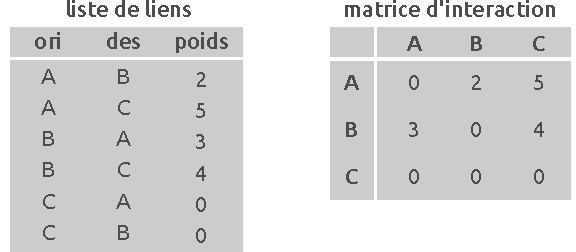
\includegraphics[width=9cm]{MatriceOD.pdf}
\end{figure}

\end{frame}



% FRAME
\begin{frame}{Network Analysis}

Leonhard Euler and the \textbf{Seven Bridges of Königsberg} (Kaliningrad).


\begin{figure}
  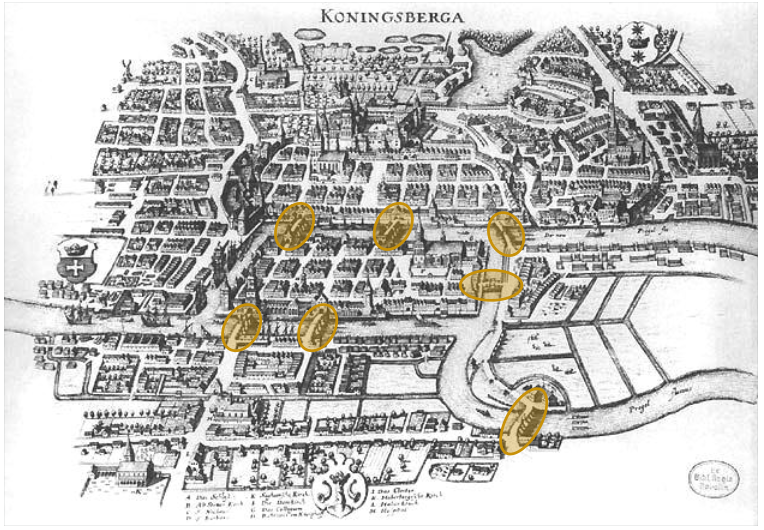
\includegraphics[width=10cm]{Konigsberg.png}
\end{figure}

\end{frame}


% FRAME
\begin{frame}{Network analysis}

\begin{figure}
  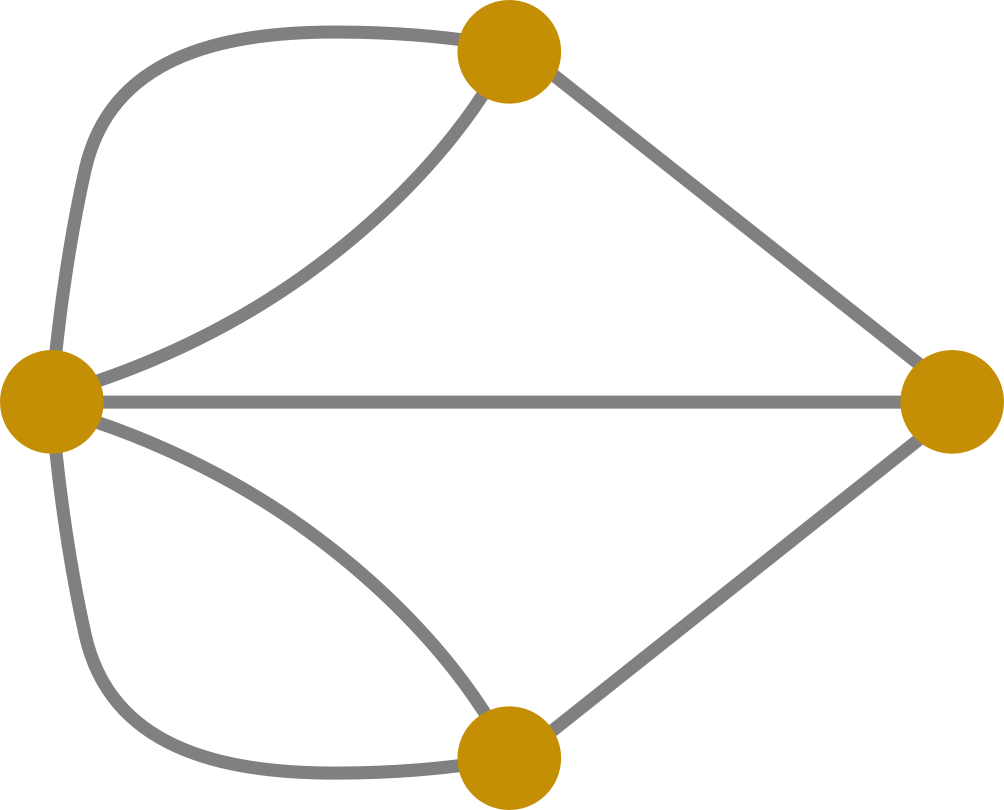
\includegraphics[width=5cm]{Konigsberg_graph.png}
\end{figure}

~

\begin{itemize}
\item No \textbf{cycle eulérien} (parité des liens incidents)
\item Pas de \textbf{chaîne eulérienne} (continuité du tracé)
\end{itemize}


\end{frame}



% FRAME
\begin{frame}{Graphs}

A graph is a set of \textit{vertices}) connected by \textbf{edges}.



Examples:

\begin{itemize} 
  \item \textbf{Transportation networks  :} e.g. Subway: nodes are  stations,  edges are lines.
  \item \textbf{Social networks:} individuals (nodes) , social interactions (edges)
  \item \textbf{Scientific collaboration networks:} Co-autorship (edges) among researchers (nodes)
  \item \ldots
\end{itemize}

\end{frame}




% FRAME
\begin{frame}{Types of graphs}

\textbf{Undirected graph:}

\begin{figure}
  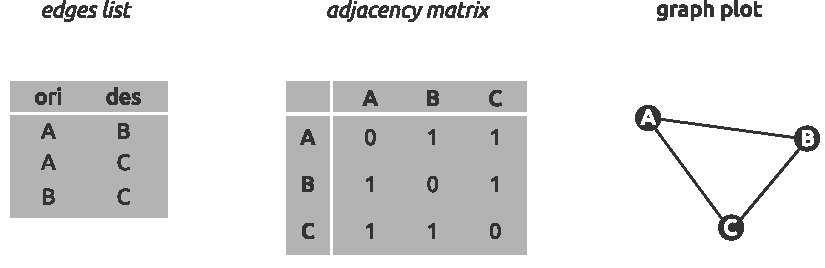
\includegraphics[width=12cm]{MatGraph3_EN.pdf}
\end{figure}

\end{frame}


% FRAME
\begin{frame}{Types of graphs}

\textbf{Directed graph :}

\textit{arcs} are employed instead of \textit{edges} who are "undirected".

\begin{figure}
  \includegraphics[width=12cm]{MatGraph2_EN.pdf}
\end{figure}

\end{frame}



% FRAME
\begin{frame}{Types of graphs}

\textbf{Weighted directed graph:}

\begin{figure}
  \includegraphics[width=12cm]{MatGraph1_EN.pdf}
\end{figure}

Also :
\begin{itemize}
  \item Weighted undirected graphs
  \item Multi-graph ()
  \item Multi-partite graphs (several types of nodes )
  \item Hypergraphs (links between more than 2 nodes)
  \item \ldots
\end{itemize}

\end{frame}





% FRAME
\begin{frame}{Network analysis : measures}

\textbf{Global measures:}

\begin{itemize}
\item number of nodes
\item number of edges
\item (number of) connected components
\item Density (ratio between nodes and edges)
\item Diameter : max length among shortest paths 
\item Connectivity : ratio between number of edges and possible number of edges
\end{itemize}

~

$\rightarrow$ \textbf{Maximum number of edges (no loops) :}

\begin{itemize}
\item Planar graph : $3V - 6$
\item Undirected non-planar graph: $\frac{V(V-1)}{2}$ 
\item  Directed non-planar graph : $V(V-1)$
\end{itemize}

\end{frame}

% FRAME
\begin{frame}{Network analysis measures}

\textbf{Nodes measures:}

\begin{itemize}
\item Degree: number of edges (neighbors) of a node 
\item in-degree / out-degree : number of inomling arcs / outgoing arcs
\item Weighted degree : sum of edges wights
\item Closeness centrality:  inverse of the sum of the shorstest paths length to any other node in the graph
\item Betweenness centrality: number of shortest paths between any two vertices of the graph that contain the node.
\end{itemize}

\end{frame}


%FRAME
\begin{frame}{Distances in Network}

In a connected graph, there is many (an infinity) paths connecting one node to every other node. 


\begin{figure}
  \includegraphics[width=5cm]{Konigsberg_graph.png}
\end{figure}


The \textbf{shortest} of these paths is adopteed as a «\textbf{network distance}» indicator.

\end{frame}

%FRAME
\begin{frame}{Djikstra Algorithm principles }

Djikstra (1959) proposed a breadth-first algorithm for directed weighted graphs, to compute the shortest path between a node and the others

~

Given $G(V,E)$ a graph, 

$V_{orig} \in V$  a node,

$w(a,b)$ a function giving the weight of the edeges linking vertices $a$ and $b$ (or $+\infty$ if none)

~ 

\begin{itemize}
\item The algorithm builds $P$ , a \textit{sub-graph} of $G$ so that any distance from $V_{orig}$ to a node $a\in P$ is known and minimum in $G$

\item A Distance list from $V_{orig}$ to any $v \in V $ are maintained. Distance of a given path is the sum of its edges weights 

\item $P$ grows by adding an edge $(a,b)$ of $P\times G $ if $d(V_{orig}, b)$ is minimum. 

\item Algorithm terminates when $P$ is a \textit{minimum spanning tree}, i.e. a tree visiting every node with a minimal sum of edges weights.
\end{itemize}
~


(Also works on undirected graphs, and for a given $V_{dest}$ destination node)



\end{frame}



%FRAME
\begin{frame}{Djikstra's pseudo code}

Init 

$P \leftarrow \emptyset $

$d(v) := 0 , \forall v \in V$ (distances to $V_{orig}$)


$d(V_{orig}) :=0$

~

While $\exists v \in V$ such that $v\notin P$:

\hspace{1cm} pick a node $a \notin P$ such that $d(a)$ is minimum

\hspace{1cm} add $a$ to $P$

\hspace{1cm} For each $ b \notin P$ such that $w(a,b) \neq \infty $

\hspace{2cm} $d(b)=min(d(b),d(a)+w(a,b))$

\hspace{1cm} End for each

End While

\end{frame}


%FRAME
\begin{frame}


A good  visualization is available at :
 
\small
 \url{https://www.cs.usfca.edu/~galles/visualization/Dijkstra.html}
\end{frame}



\begin{comment}

% FRAME
\begin{frame}{Distance and Interaction}

Spatial interactions imply \textbf{distance}.

~

\begin{itemize}
  \item Spatial interaction considers \textbf{ travel as an effort }.
  \item Spatial interaction confront \textbf{connecting entities} and the \textbf{distance induced decay}.
  \item Spatial interaction comes in two flavors : \textbf{relationships between locations}  or \textbf{attraction/influence of a location on the others}. 
  \begin{itemize}
  \item The first relies on \textbf{flow analysis}
  \item The second relies on \textbf{position analysis}(\textit{ Accessibility})
  \end{itemize}
\end{itemize}

\end{frame}


% FRAME
\begin{frame}{What is distance ?}


\textbf{In Geography}, distance is a separation, requiring \textbf{effort} to be crossed. Distance is a \textbf{friction}, a barrier:

\begin{itemize}
  \item \emph{«Everything is related to everything else, but near things are more related than distant things»} (Tobler)
\end{itemize}

~ 

\textbf{In Maths}, a distance is a function satisfying the following conditions 

\begin{itemize}
  \item Symmetry $d(a, b) = d(b,a)$
  \item Identity of indicernibles : $d(a, b) = 0 \Longleftrightarrow a = b$
  \item Triangle inequality: $d(a,c) \leq d(a,b) + d(b,c)$
\end{itemize}

\end{frame}


% FRAME
\begin{frame}{Euclidean Distance }


\textbf{For a n-dimensional vector:}

\begin{equation}
  \nonumber
  d(a,b) = \sqrt{\sum_{i=1}^n (a_i - b_i)^2}
\end{equation}

\end{frame}


% FRAME
\begin{frame}{Manhattan Distance}

\textbf{2D vector : }

\begin{figure}
  \includegraphics[width=8cm]{DistancesMan.pdf}
\end{figure}

\textbf{For a n-dimensional vector:}

\begin{equation}
  \nonumber
  d(a,b) = \sum_{i=1}^n |a_i - b_i|
\end{equation}

\end{frame}






% FRAME
\begin{frame}{Flow modeling}

\textbf{Original gravity model:}

\begin{equation}
\nonumber
T_{ij} = k \frac{P_i P_j}{D_{ij}^{2}}
\end{equation}

~
With $T_{ij}$, the flow from location $i$ to $j$.

$k$ a constant

$P_i$ the mass of location $i$

$D_{ij}$ the distance between location $i$ and $j$.


~

Many variations exist according to the choice of the terms:

\begin{itemize}
  \item \textbf{Masses:} populations, jobs , emissions, attractions
  \item \textbf{Masses weights:} multiplying factors or exponents
  \item \textbf{Friction function (distance):} negative powers, negative exponent
  \item \textbf{Margin Constraints:} double, simple, none
  \item \textbf{Numeric Resolution } 
\end{itemize}


\end{frame}


% FRAME
\begin{frame}{Modélisation des flux: formalisation}

\textbf{Le modèle d'opportunités interposées} (Stouffer 1960) s'écrit:

\begin{equation}
\nonumber
T_{ij} = k_i O_i \left[\exp(-\alpha x_{j-1}) - \exp(-\alpha x_{j}) \right]
\end{equation}

~

\textbf{Le modèle de radiation} (Simini \textit{et al.} 2012) s'écrit:  

\begin{figure}
  \includegraphics[width = 110mm]{CercleStouffer.pdf}
\end{figure}

\end{frame}


\end{comment}
  

%\section{Accessibility}

 %% Définition du répertoire contenant les images
\graphicspath{{IMAGE/}}


% FRAME Intro
\begin{frame}

\includegraphics[width=12cm]{Logos.pdf}

\vfill

\begin{center}

\vspace*{1.5cm}

\LARGE
\textbf{Accessibility}

\vspace*{1.5cm}
 DELHI GIS-R School


\large
9-12\up{th} April 2019

\vspace*{1.5cm}


\textbf{Hadrien Commenges \& Paul Chapron}

{\small

\vspace*{0.1cm}

\url{hadrien.commenges@univ-paris1.fr}

\url{paul.chapron@ign.fr}
}

\end{center}

\end{frame}


% FRAME
\begin{frame}{Use case}


\begin{block}{Accessibility}
Accessibility depicts the potential access of an agent to a resource.

\end{block}

\textbf{two meanings:}

\begin{enumerate}
  \item \textbf{Access to a location:} required effort for agents to get to a location ($\approx$ service area).Such a measure depends on the network (infrastructure + services) and the agent's capacity to travel.
  \item \textbf{Access to a resource:} required effort for agents to get to a resource. Suche a measure depends on the network, the agent's capacity to travel and the resource \textbf{spatial distribution}.
\end{enumerate}

~

~

\textbf{What kind of geographical information is concerned ?}

$\rightarrow$ \textit{TYPE 1 - Geographical Objects}

$\rightarrow$ \textit{TYPE 2 - Occurrences}

$\rightarrow$ \textit{TYPE 3 - Measure points}

$\rightarrow$ \textit{TYPE 4 - Statistics}

$\rightarrow$ \textit{TYPE 5 - Interaction Measures}


\end{frame}



% FRAME
\begin{frame}{Distance and interaction}

\begin{itemize}
  \item \textbf{friction} (\textit{impedance}) is the key-concept, distance is a measure of friction.
  \item Spatial interaction is adressed via \textbf{interactions between locations} (flows) or \textbf{attraction/influence of a location on the others}. 
  \item Accessibility models rely on the latter.
\end{itemize}

\end{frame}



\section{Concentration, Segregation, Autocorrelation}
  
% Définition du répertoire contenant les images
\graphicspath{{IMAGE/}}

% FRAME Intro
\begin{frame}

\includegraphics[width=12cm]{Logos.pdf}

\vfill

\begin{center}

\vspace*{1.5cm}

\LARGE
\textbf{Concentration, Segregation, Autocorrelation}

\vspace*{1.5cm}
 DELHI GIS-R School


\large
9-12\up{th} April 2019

\vspace*{1.5cm}


\textbf{Hadrien Commenges \& Paul Chapron}

{\small

\vspace*{0.1cm}

\url{hadrien.commenges@univ-paris1.fr}

\url{paul.chapron@ign.fr}
}

\end{center}

\end{frame}

% FRAME
\begin{frame}{A good starting point}

\textbf{Information about tools and methods }

~

GeoDa Center for Geospatial Analysis and Computation (Luc Anselin)

\url{https://geodacenter.asu.edu}

~

$\rightarrow$ logiciels \emph{standalone} (GeoDa) + Python and  R libraries \\
$\rightarrow$ tutorials, references, online courses


\end{frame}


% FRAME
\begin{frame}{Concentration}

\textbf{Classical methods from inequality economics}

\begin{figure}
\includegraphics[width=12cm]{Inequalities.jpg}
\end{figure}

\end{frame}


% FRAME
\begin{frame}{Concentration}

\textbf{Hoover  index} \\
\emph{(Dissimilarity index} or \emph{Duncan's I)}

~

For two classes $x$ and $y$ of a population  that sum up to 100\% (e.g. male / female), 

\begin{equation}
\nonumber
H = \frac{1}{2} \sum_{i=1}^n \bigg| \frac{x_i}{x_{tot}} - \frac{y_i}{y_{tot}} \bigg|
\end{equation}


(also the longest vertical distance between the lorenz Curve and the 45 degrees line of perfect equality)

\end{frame}


% FRAME
\begin{frame}{Concentration}
\begin{figure}
\includegraphics[width=9cm]{Gateau2_EN.pdf}
\end{figure}

\end{frame}



% FRAME
\begin{frame}{Concentration}

\textbf{Gini index}

~

relative mean of absolute differences between every pair of a stock 

\begin{equation}
\nonumber
G = \frac{\sum_i \sum_j |x_i - x_j|}{2n \sum_i x_i}
\end{equation}


ranges from 0 (perfect equality) to 1 (perfect inequality), but these theoretical values are never reached.





\end{frame}	



% FRAME
\begin{frame}{Concentration}


%TODO figure EN 
\begin{figure}
\includegraphics[width=12cm]{Lorenz.pdf}
\end{figure}

\end{frame}


% FRAME
\begin{frame}{Segregation}

\textbf{Entropy-based measures}

These meassures comes from the field of information theory (Shannon) ~

\textbf{Quantity of information $I$ (in bits) of a message $m$ :} logarithm (base 2) of the ratio between the finite set of every possible message before a message is recieved ($M$, the universe) and  the finite set of possible message after it is recieved ($m$):

~

\begin{equation}
\nonumber
  I = \log\left(\frac{M}{m} \right) = - \log(p(m))
\end{equation}

~

This quantity is expressed in \emph{bits} since the logarithm base is 2.

\end{frame}


% FRAME
\begin{frame}{Segregation}

\textbf{Entropy-based measures}

~ 

\textbf{I}: Information brought by the occcurence of a message (informative event) . 

\textbf{H} (entropy): information stored in a finite set of informative event (e.g. all the messages of a transmission) \\ 
- i.e. average quantity of information stored in a set of messages \\ 
- i.e. each message bring as much information as its quantity of information multiplied by its probability of apparition.

\begin{equation}
  H(x) = - \sum\limits_{i=1}^n p_i \log(p_i)
  \nonumber
\end{equation}

~

\textbf{Relative entropy:} ratio between an entropy and the maximum entropy $H_{max}$

\begin{equation}
  H_{max} = \log(n)
  \nonumber
\end{equation}

\end{frame}



% FRAME
\begin{frame}{Segregation}

\textbf{Entropy interpretation guide}

~ 

Low (relative) entropy values tend to indicate segregated configurations

~

High (relative) entropy values tend to indicate more evenly distributed configurations



\end{frame}



% FRAME
\begin{frame}{Autocorrelation}

Hoover, Gini, Shannon (Theil) indexes can't distinguish between these configurations \\ 

\begin{figure}
\includegraphics[width=12cm]{NonSpatial.pdf}
\end{figure}

Autocorrelation indexes (\textbf{Geary} and \textbf{Moran}) can distinguish between \textbf{1} et \textbf{2}.

\end{frame}


% FRAME
\begin{frame}{Autocorrelation}

Moran's I (1950):

$$
I = \frac{n}{\sum_{i} \sum_{j} w_{ij}} \times \frac{\sum_{i} \sum_{j} w_{ij} (x_i - \bar{x})(x_j - \bar{x})}{\sum_{i} (x_i - \bar{x})^2}
$$

~

$n$ : number of spatial units \\ 
$x_i$ et $x_j$ : values of $x$ in $i$ and $j$ \\ 
$\bar{x}$ : average value of $x$ \\ 
$w_{ij}$ : weighting matrix corresponding to the neighborhood definition

\end{frame}



% FRAME
\begin{frame}{Autocorrelation}

\textbf{Moran's I} interpretation based on \textbf{Moran's plot}

\begin{figure}
\includegraphics[width=12cm]{MoranPlot.pdf}
\end{figure}

\end{frame}


% FRAME
\begin{frame}{Autocorrelation}

\textbf{Local contribution to the global autocorrelation index} \\
LISA - \emph{local indicators of spatial autocorrelation}

$$
I_i = z_i \sum_{j} w_{ij} z_j
$$

~

$z_i$ standardized value of $x$ for spatial unit $i$ \\
$z_j$ standardized value of $x$ for spatial unit $j$ \\
$w_{ij}$ weighting matrix

\end{frame}


% FRAME
\begin{frame}{Spatial autoregressive model}

The autocorrelation can be used in a \textbf{descriptive} approach or in a \textbf{modeling} approach.

~

Ex. of land values modeling (econometrics): the value of a dwelling is function of:

\begin{itemize}
  \item Intrinsic attributes: surface area, garden, etc.
  \item Contextual attributes: i.e. the value of the dwellings in the neighborhood
\end{itemize}

~

In this case, it may be useful to build a \textbf{spatial autoregressive regression} (SAR), i.e. to inject the \textbf{lagged values} (neighborhood average) as a regressor.

\end{frame}




\end{document}
